\documentclass[11pt]{article}

\usepackage[a4paper]{geometry}
\geometry{left=2.0cm,right=2.0cm,top=2.5cm,bottom=2.5cm}

\usepackage{ctex} % 支持中文的LaTeX宏包
\usepackage{amsmath,amsfonts,graphicx,subfigure,amssymb,bm,amsthm,mathrsfs,mathtools,breqn} % 数学公式和符号的宏包集合
\usepackage{algorithm,algorithmicx} % 算法和伪代码的宏包
\usepackage[noend]{algpseudocode} % 算法和伪代码的宏包
\usepackage{fancyhdr} % 自定义页眉页脚的宏包
\usepackage[framemethod=TikZ]{mdframed} % 创建带边框的框架的宏包
\usepackage{fontspec} % 字体设置的宏包
\usepackage{adjustbox} % 调整盒子大小的宏包
\usepackage{fontsize} % 设置字体大小的宏包
\usepackage{tikz} % 绘制图形和使用颜色的宏包
\usetikzlibrary{arrows.meta} % TikZ箭头库
\usepackage{float} % 支持[H]浮动体位置参数
\usepackage{multicol} % 多栏排版的宏包
\usepackage{multirow} % 表格中合并单元格的宏包
\usepackage{pdfpages} % 插入PDF文件的宏包
\RequirePackage{listings} % 在文档中插入源代码的宏包
\usepackage{wrapfig} % 文字绕排图片的宏包
\usepackage{bigstrut,multirow,rotating} % 支持在表格中使用特殊命令的宏包
\usepackage{booktabs} % 创建美观的表格的宏包
\usepackage{circuitikz} % 绘制电路图的宏包
\usepackage{hyperref} % 创建超链接的宏包

\definecolor{dkgreen}{rgb}{0,0.6,0}
\definecolor{gray}{rgb}{0.5,0.5,0.5}
\definecolor{mauve}{rgb}{0.58,0,0.82}
\lstset{
  frame=tb,
  aboveskip=3mm,
  belowskip=3mm,
  showstringspaces=false,
  columns=flexible,
  framerule=1pt,
  rulecolor=\color{gray!35},
  backgroundcolor=\color{gray!5},
  basicstyle={\small\ttfamily},
  numbers=none,
  numberstyle=\tiny\color{gray},
  keywordstyle=\color{blue},
  commentstyle=\color{dkgreen},
  stringstyle=\color{mauve},
  breaklines=true,
  breakatwhitespace=true,
  tabsize=3,
}


\usepackage[capitalize]{cleveref}
\Crefname{section}{Section}{Sections}
\Crefname{table}{Table}{Tables}
\crefname{table}{Table.}{Tabs.}

\setmainfont{Palatino Linotype}
\setCJKmainfont{SimSun}[BoldFont=SimHei, ItalicFont=KaiTi]
\setCJKsansfont{SimHei}
\setCJKmonofont{FangSong}
\punctstyle{kaiming}
% 偏好的几个字体, 可以根据需要自行加入字体ttf文件并调用

% Restore standard emphasis to avoid requiring an undefined environment (kaishu).
% The original redefinition used an environment `kaishu` which is not defined
% in a default ctex setup and causes compilation errors. Use \textit for
% emphasis which works across engines.
\renewcommand{\emph}[1]{\textit{#1}}

%改这里可以修改实验报告表头的信息
\newcommand{\experiName}{杨氏模量}
\newcommand{\supervisor}{边苓竹}
\newcommand{\name}{邓思豪}
\newcommand{\studentNum}{2023K8009909008}
\newcommand{\class}{3}
\newcommand{\group}{01}
\newcommand{\seat}{5}
\newcommand{\dateYear}{2025}
\newcommand{\dateMonth}{10}
\newcommand{\dateDay}{15}
\newcommand{\room}{学院二340}
\newcommand{\others}{$\square$}


\begin{document}



\begin{center}
    \LARGE \bf 《\, 基\, 础\, 物\, 理\, 实\, 验\, 》\, 实\, 验\, 报\, 告
\end{center}

\begin{center}
    \noindent \emph{实验名称}\underline{\makebox[25em][c]{\experiName}}
    \emph{指导教师}\underline{\makebox[8em][c]{\supervisor}}\\
    \emph{姓名}\underline{\makebox[6em][c]{\name}} 
    % 如果名字比较长, 可以修改box的长度"6em"
    \emph{学号}\underline{\makebox[10em][c]{\studentNum}}
    \emph{分班分组及座号} \underline{\makebox[5em][c]{\class \ -\ \group \ -\ \seat }\emph{号}} （\emph{例}:\, 1\,-\,04\,-\,5\emph{号}）\\
    \emph{实验日期} \underline{\makebox[3em][c]{\dateYear}}\emph{年}
    \underline{\makebox[2em][c]{\dateMonth}}\emph{月}
    \underline{\makebox[2em][c]{\dateDay}}\emph{日}
    \emph{实验地点}\underline{{\makebox[6em][c]\room}}
    \emph{调课/补课} \underline{\makebox[3em][c]{\others\ 是}}
    \emph{成绩评定} \underline{\hspace{5em}}
    {\noindent}
    \rule[8pt]{17cm}{0.2em}
\end{center}

\section{实验目的}

\begin{enumerate}
    \item 理解各种静态方法测杨氏模量及其测量微小位移方法的原理及优缺点，了解动态法测 杨氏模量的原理。
    \item 熟悉霍尔位置传感器的特性，完成样品的测量和对霍尔位置传感器定标，理解传感器 特定曲线对测量的意义。
    \item 了解光杠杆法的放大原理和适用条件。
    \item 学会读数望远镜、读数显微镜的调节。
    \item 学习用逐差法、作图法和最小二乘法处理数据。
    \item 学会计算各物理量的不确定度，并用不确定度正确表达实验结果。
\end{enumerate}

\section{实验器材}
\subsection*{2.1拉伸法测定金属的杨氏模量}
\begin{enumerate}
    \item CCD杨氏弹性模量测量仪（LB-YM1型、YMC-2型），螺旋测微器（分度值：0.01mm 量程：0~25mm），钢卷尺（量程：3m，最小分度值1mm）。
（注意事项：测量仪的金属丝必须保持铅直形态。测直径时要特别谨慎，避免由于扭转、拉扯、牵挂导致细丝折弯边形。）
\end{enumerate}
\subsection*{2.2使用霍尔传感器测杨氏模量（弯曲法）}
\begin{enumerate}
    \item 读数显微镜：型号JC-10型 目镜放大率10X 目镜测微鼓轮最小分度值 0.01mm 物镜放大率2X 测量范围 0~6mm 鼓轮实际读数最小分辨率0.01/2=0.005mm 
    \item 电子秤传感器加力系统：0~199.9g连续可调，三位半数显。
    \item 霍尔电压表： 量程1:   0~199.9mV，分辨率0.1mV；量程2：0~1.999V，分辨率1mV
    \item 霍尔位置传感器：灵敏度大于250mV/mm，线性范围0~2mm。
    \item 螺旋测微计：分度值0.01mm，测量范围0~25mm。
    \item 卷尺：钢尺，量程30cm，最小分度值0.5mm
\end{enumerate}
\subsection*{2.3 动态悬挂法测杨氏模量}
\begin{enumerate}
    \item DHY-2A型动态杨氏模量测试台，DH0803振动力学通用信号源，通用示波器，测试棒（铜、不锈钢），悬线，专用连接导线，天平，游标卡尺，螺旋测微计。
    \item 注意事项：安装测试棒时，应先移动支架到既定位置，再悬挂测试棒；更换测试棒要细心，避免损坏激振，共振传感器。
\end{enumerate}

\section{数据的不确定度}

本次实验的一大重点就是理解并掌握数据的有效数字及不确定度的计算与合成，
故专门开一小节讨论。

\subsection*{3.1 \ 不确定度 $\Delta N$}

不确定度是定量表征测量值分散性的参数，用以描述测量结果的可靠程度与精确水平。它反映了测量值相对于真值可能存在的偏离范围，是评价测量结果质量的重要指标。在物理实验中，任何测量都不可避免地存在误差，因此完整的测量结果应表示为$Y=N\pm\Delta N$的形式，其中$N$为测量的最佳估计值，$\Delta N$为测量的不确定度。此外，为了便于比较不同量级测量结果的精度，常引入相对不确定度的概念，定义为$u_r=\Delta N/N$，它是一个无量纲量，能够更直观地反映测量的相对精确程度。

\subsection*{3.2 \ 两类不确定度（A 类与 B 类）}

根据不确定度评定方法的不同，可将其分为A类不确定度和B类不确定度两大类型。这种分类方法主要依据于获取不确定度的途径：通过统计分析得到的为A类，通过其他方法估计得到的为B类。

\textbf{A类不确定度} $u_A(x)$：这是一种通过对测量数据进行统计分析而得到的不确定度分量，主要反映在相同测量条件下进行多次重复测量时，由于随机因素（如环境波动、读数随机性等）导致的测量值分散程度。A类不确定度也称为测量列的标准偏差或实验标准偏差，其数学表达式为：
\begin{equation}
   u_A(x)=\sqrt{\frac{\sum_{i=1}^n(x_i-\overline x)^2}{n(n-1)}}
\end{equation}
式中，$x_i$为第$i$次测量值，$\overline x$为$n$次测量的算术平均值，$n$为测量次数。该公式体现了贝塞尔公式的统计学原理。

\textbf{B类不确定度} $u_B(x)$：这是通过非统计方法评定的不确定度分量，通常基于经验、仪器规格说明书、检定证书等信息进行估算。B类不确定度可进一步细分为两个组成部分：

（1）单次测量时的估读不确定度$u_{B1}(x)$：由于人眼判读仪器刻度时存在主观估计，一般根据测量者的估读能力取为仪器最小分度值$d$的一定比例。常见的取值方式有$d$、$\frac{d}{10}$或$\frac{d}{5}$，具体取值取决于仪器的刻度清晰度和测量者的熟练程度。

（2）仪器不确定度$u_{B2}(x)$：由仪器本身的制造精度、校准精度等因素引起，通常取仪器的最大允许误差（允差）$e$除以$\sqrt{3}$，即：
\begin{align}
   u_{B1}(x)&=d,\ \frac{d}{10},\ \frac{d}{5}\notag\\
   u_{B2}(x)&=\frac{e}{\sqrt 3} 
\end{align}

在本次实验中，考虑到实验仪器的精度特点和测量者的估读水平，采用$u_{B1}(x)=\frac{d}{10}$的评定方式，其中$d$为仪器的最小分度值，$e$为仪器说明书或检定证书中标注的最大允许误差（允差）。

\subsection*{3.3 \ 不确定度的合成}

在实际测量中，多种不确定度来源往往同时存在，因此需要将各个独立的不确定度分量按照一定规则合成为总不确定度。根据误差传播理论，当各不确定度分量相互独立时，采用方和根的方法进行合成。

\textbf{单次测量的情况}：当仅进行一次测量时，不存在统计分散性，因此总不确定度仅由B类不确定度的两个分量合成：
\begin{equation}
    u(x)=\sqrt{u_{B1}^2(x)+u^2_{B2}(x)} 
\end{equation}

\textbf{长度测量的特殊情况}：在长度测量中，测量结果通常是两个端点读数之差，因此需要考虑两次读数各自的估读不确定度。此时估读不确定度$u_{B1}(x)$需要计入两次，合成公式修正为：
\begin{equation}
    u(x)=\sqrt{u_{B1}^2(x)+u_{B1}^2(x)+u^2_{B2}(x)} =\sqrt{2u_{B1}^2(x)+u^2_{B2}(x)} 
\end{equation}
这体现了长度差值测量中两个端点读数误差的独立叠加效应。

\textbf{多次测量的情况}：当进行多次重复测量时，既存在随机因素引起的A类不确定度，也存在仪器系统因素引起的B类不确定度（此时单次估读不确定度已被A类不确定度包含，不再单独计入）。总不确定度的合成公式为：
\begin{equation}
   u(x)=\sqrt{u_A^2(x)+u^2_{B2}(x)} 
\end{equation}
这种合成方式充分考虑了统计分散性和仪器系统误差的共同作用，能够更全面地反映测量结果的不确定性。




\section{实验原理}
\subsection*{4.1 拉伸法}
物体在外力作用下都会发生形变。当形变在一定限度内，撤走外力能恢复原状的形变称为弹性形变。
反之撤走外力之后仍有剩余形变，称为塑性形变。发生弹性形变时，弹性模量便是反应材料形变与内应力关系的基本物理量。

设柱状物体的长度为$L$，截面积为$S$，沿长度方向受外力$F$作用后伸长（或缩短）量为$\Delta L$，单位横截面积上垂
直作用力$F/S$称为正应力，物体的相对伸长$\Delta L/L$称为线应变。胡克定律告诉我们：
\begin{equation}
   F/S=Y\frac{\Delta L}{L} 
\end{equation}
其中$Y$便称为杨氏模量，本实验中我们将以显微镜和CCD成像系统进行对$\Delta L$的测量，并通过砝码测量外力，通过钢卷尺测量金属丝长度，
通过螺旋测微器测量金属丝直径，从而将知道有公式：
\begin{equation}
    Y=\frac{4FL}{\pi d^2\Delta L}
\end{equation}
\subsection*{4.2 霍尔传感器弯曲法}
\begin{enumerate}
    \item 霍尔位置传感器原理
当保持霍尔元件的电流$I$不变，并使其在均匀梯度磁场中移动时，输出的霍尔电势差变化量为：
\begin{equation}
\Delta U_H = K \cdot I \cdot \frac{dB}{dZ} \cdot \Delta Z
\label{eq:hall_position}
\end{equation}

其中，$\frac{dB}{dZ}$为磁感应强度沿位移方向的变化率（磁场梯度），$\Delta Z$为位移量。

当磁场梯度$\frac{dB}{dZ}$为常数时，$\Delta U_H$与$\Delta Z$成正比，即：
\begin{equation}
\Delta U_H \propto \Delta Z
\end{equation}

这意味着通过测量霍尔电势差的变化，可以精确测定微小位移量。当位移量较小（一般小于2mm）时，这种对应关系具有良好的线性特性。\par

均匀梯度磁场的实现
为实现均匀梯度磁场，实验通常采用两块相同的磁铁平行相对放置（N极相对），两磁铁之间留有等间距间隙。霍尔元件平行于磁铁放置在间隙的中轴上。间隙中心截面处的磁感应强度为零，当霍尔元件处于此位置时，输出的霍尔电势差为零，此位置可作为位移参考零点。

\begin{figure}[H]
\centering
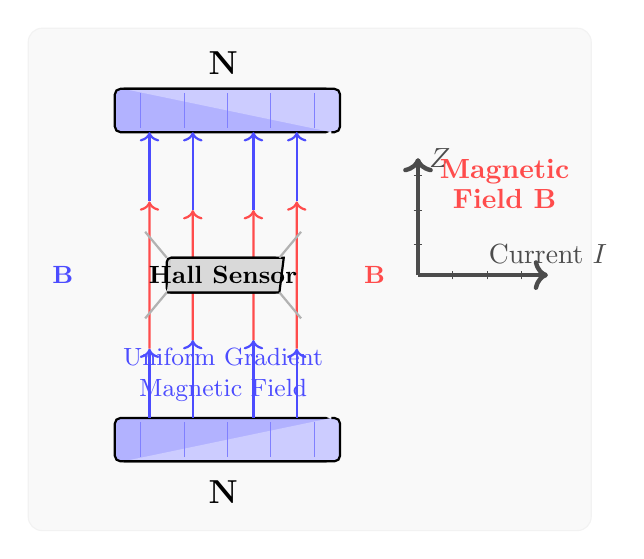
\begin{tikzpicture}[scale=1.1]
% 背景淡色框
\draw[gray!10, fill=gray!5, rounded corners=5pt] (-1,-0.8) rectangle (5.5,5);

% 上方磁铁（带立体感和圆角）
\draw[thick, fill=blue!30, rounded corners=2pt] (0,3.8) rectangle (2.5,4.3);
\draw[thick, fill=blue!20, rounded corners=2pt] (0.1,4.3) -- (2.6,4.3) -- (2.6,3.8) -- (2.5,3.8);
% 磁铁表面细节
\foreach \x in {0.3,0.8,1.3,1.8,2.3} {
    \draw[blue!50, thin] (\x,3.85) -- (\x,4.25);
}
\node at (1.25,4.6) {\large\textbf{N}};

% 下方磁铁（带立体感和圆角）
\draw[thick, fill=blue!30, rounded corners=2pt] (0,0) rectangle (2.5,0.5);
\draw[thick, fill=blue!20, rounded corners=2pt] (0.1,0) -- (2.6,0) -- (2.6,0.5) -- (2.5,0.5);
% 磁铁表面细节
\foreach \x in {0.3,0.8,1.3,1.8,2.3} {
    \draw[blue!50, thin] (\x,0.05) -- (\x,0.45);
}
\node at (1.25,-0.35) {\large\textbf{N}};

% 磁场线（优化位置，更加均匀）
\draw[->, thick, blue!70] (0.4,0.5) -- (0.4,1.3);
\draw[->, thick, blue!70] (0.4,3.0) -- (0.4,3.8);
\draw[->, thick, red!70] (0.4,1.3) to[out=90,in=270, looseness=0.8] (0.4,3.0);

\draw[->, thick, blue!70] (0.9,0.5) -- (0.9,1.4);
\draw[->, thick, blue!70] (0.9,2.9) -- (0.9,3.8);
\draw[->, thick, red!70] (0.9,1.4) to[out=90,in=270, looseness=0.6] (0.9,2.9);

\draw[->, thick, blue!70] (1.6,0.5) -- (1.6,1.4);
\draw[->, thick, blue!70] (1.6,2.9) -- (1.6,3.8);
\draw[->, thick, red!70] (1.6,1.4) to[out=90,in=270, looseness=0.6] (1.6,2.9);

\draw[->, thick, blue!70] (2.1,0.5) -- (2.1,1.3);
\draw[->, thick, blue!70] (2.1,3.0) -- (2.1,3.8);
\draw[->, thick, red!70] (2.1,1.3) to[out=90,in=270, looseness=0.8] (2.1,3.0);

% 霍尔元件（中心位置）
\draw[thick, fill=gray!40, rounded corners=1.5pt] (0.6,1.95) rectangle (1.9,2.35);
\draw[thick, fill=gray!30] (0.65,2.35) -- (1.95,2.35) -- (1.9,1.95) -- (0.6,1.95);
% 元件引脚
\draw[thick, gray!60] (0.6,1.95) -- (0.35,1.65);
\draw[thick, gray!60] (1.9,1.95) -- (2.15,1.65);
\draw[thick, gray!60] (0.6,2.35) -- (0.35,2.65);
\draw[thick, gray!60] (1.9,2.35) -- (2.15,2.65);
\node at (1.25,2.15) {\small\textbf{Hall Sensor}};

% 坐标轴系统（移到右侧，避免遮挡）
\draw[->, ultra thick, black!70] (3.5,2.15) -- (3.5,3.5) node[right] {$Z$};
\draw[black!70] (3.45,2.5) -- (3.55,2.5);
\draw[black!70] (3.45,2.9) -- (3.55,2.9);
\draw[black!70] (3.45,3.3) -- (3.55,3.3);

\draw[->, ultra thick, black!70] (3.5,2.15) -- (5,2.15) node[above] {Current $I$};
\draw[black!70] (3.9,2.1) -- (3.9,2.2);
\draw[black!70] (4.3,2.1) -- (4.3,2.2);
\draw[black!70] (4.7,2.1) -- (4.7,2.2);

% 标注（优化位置）
\node[red!70, align=center] at (4.5,3.2) {\textbf{Magnetic}\\[-1pt]\textbf{Field $\mathbf{B}$}};
\node[blue!70, align=center] at (1.25,1.0) {\small Uniform Gradient\\[-1pt]\small Magnetic Field};

% 标注磁场方向
\node[blue!70] at (-0.6,2.15) {\small $\mathbf{B}$};
\node[red!70] at (3.0,2.15) {\small $\mathbf{B}$};

\end{tikzpicture}
\caption{霍尔位置传感器在均匀梯度磁场中的工作原理示意图}
\label{fig:hall_sensor}
\end{figure}
\item 杨氏模量在弯曲法中的测量的公式推导
\begin{figure}[H]\centering
    \resizebox{!}{160pt}{
        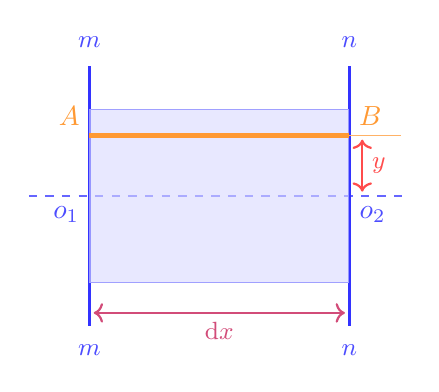
\begin{tikzpicture}[scale=1.1]
            % 中性轴（虚线）
            \draw[dashed, thick, blue!60] (-2.2,0)--(-1.5,0) node[below left, blue!70]{$o_1$}--(1.5,0) node[below right, blue!70]{$o_2$}--(2.2,0);
            
            % 两侧边界线
            \draw[very thick, blue!80] (-1.5,-1.5)--(-1.5,1.5);
            \draw[very thick, blue!80] (1.5,-1.5)--(1.5,1.5);
            
            % 微元矩形上下边界
            \draw[blue!70] (-1.5,-1)--(1.5,-1);
            \draw[blue!70] (-1.5,1)--(1.5,1);
            
            % 填充微元区域
            \fill[blue!15, fill opacity=0.6] (-1.5,-1) rectangle (1.5,1);
            
            % dx 标注
            \draw[<->, thick, purple!70] (-1.45,-1.35)--(1.45,-1.35);
            \node[below, purple!70, font=\small] at(0,-1.35) {$\mathrm{d}x$};
            
            % m, n 标注
            \node[below, blue!70, font=\small] at(-1.5,-1.6) {$m$};
            \node[below, blue!70, font=\small] at(1.5,-1.6) {$n$};
            \node[above, blue!70, font=\small] at(-1.5,1.6) {$m$};
            \node[above, blue!70, font=\small] at(1.5,1.6) {$n$};
            
            % AB线段（橙色加粗）
            \draw[line width=2pt, orange!80] (-1.5,0.7)--(1.5,0.7);
            \node[above left, orange!80, font=\bfseries] at(-1.5,0.7) {$A$};
            \node[above right, orange!80, font=\bfseries] at(1.5,0.7) {$B$};
            
            % 延长线和y标注
            \draw[orange!60] (1.5,0.7)--(2.1,0.7);
            \draw[<->, thick, red!70] (1.65,0.05)--(1.65,0.65);
            \node[right, red!70, font=\small] at(1.65,0.35) {$y$};
        \end{tikzpicture}
    }\hspace*{1.5cm}
    \resizebox{!}{160pt}{
        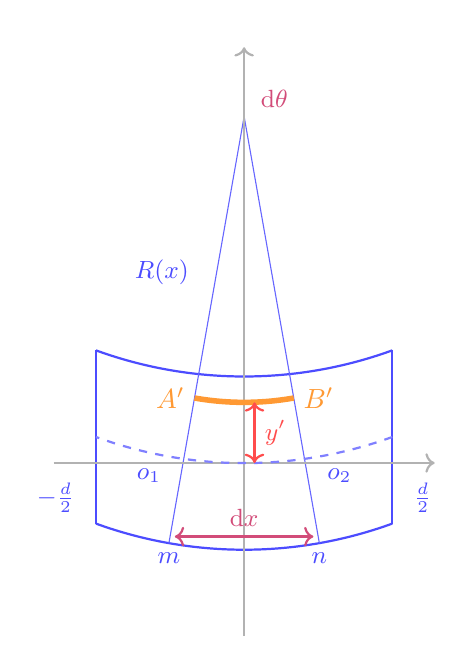
\begin{tikzpicture}[scale=1.1]
            % 弯曲后的外轮廓
            \draw[thick, blue!70] (1.71,0.3) arc (290:250:5);
            \draw[thick, blue!70] (1.71,2.3) arc (290:250:5);
            
            % 两侧边界
            \draw[thick, blue!70] (1.71,0.3)--(1.71,2.3);
            \draw[thick, blue!70] (-1.71,0.3)--(-1.71,2.3);
            
            % 从底部到顶点的线
            \draw[blue!60] (0.8682,0.0760) node[below, blue!70, font=\small]{$n$} -- (0,5);
            \draw[blue!60] (-0.8682,0.0760) node[below, blue!70, font=\small]{$m$} -- (0,5);
            
            % 坐标轴
            \draw[->, thick, gray!60] (0,-1)--(0,5.8) node[above, font=\small]{};
            \draw[->, thick, gray!60] (-2.2,1)--(2.2,1);
            
            % 中性层虚线
            \draw[dashed, thick, blue!50] (1.71,1.3) arc (290:250:5);
            
            % dx标注
            \draw[<->, thick, purple!70] (-0.8,0.15)-- node[above, font=\small]{$\mathrm{d}x$} (0.8,0.15);
            
            % d/2 标注
            \node[right, blue!70, font=\small] at(1.85,0.6) {$\frac{d}{2}$};
            \node[left, blue!70, font=\small] at(-1.85,0.6) {$-\frac{d}{2}$};
            
            % o1, o2 标注
            \node[blue!70, font=\small] at(-1.1,0.85) {$o_1$};
            \node[blue!70, font=\small] at(1.1,0.85) {$o_2$};
            
            % R(x) 标注
            \node[blue!70, font=\small] at(-0.95,3.2) {$R(x)$};
            
            % dθ 标注
            \node[purple!70, font=\small] at(0.35,5.2) {$\mathrm{d}\theta$};
            
            % A'B' 橙色弧线
            \draw[line width=2pt, orange!80] (0.573,1.7501) arc (280:260:3.3);
            \node[left, orange!80, font=\bfseries] at(-0.573,1.7501) {$A'$};
            \node[right, orange!80, font=\bfseries] at(0.573,1.7501) {$B'$};
            
            % y' 标注
            \draw[<->, thick, red!70] (0.12,1)-- node[right, font=\small]{$y'$} (0.12,1.7);
        \end{tikzpicture}
    }
    \caption{弯曲法测杨氏模量原理示意图}
\end{figure}
$o_1o_2$所在平面为中性面，既不拉伸也不压缩，$AB$为距中性面距离$y$处的平面。变形前$o_1o_2=AB=\mathrm{d}x$，变形后$o_1o_2=R(x)\mathrm{d}\theta$，$A'B'=(R(x)-y)\mathrm{d}\theta$。

则$AB$面的应变为
\begin{equation}
\varepsilon=\frac{A'B'-AB}{AB}=\frac{(R(x)-y)\mathrm{d}\theta-\mathrm{d}x}{\mathrm{d}x}=-\frac{y}{R(x)}
\end{equation}

由胡克定律$\frac{\mathrm{d}F}{\mathrm{d}S}=Y\varepsilon$，对中性面的转矩微元为
\begin{equation}\label{2-1}
    \mathrm{d}\mu(x)=\frac{Yb}{R(x)}y^2\mathrm{d}y
\end{equation}

积分得
\begin{equation}
\mu(x)=\int_{-a/2}^{a/2}\frac{Yb}{R(x)}y^2\mathrm{d}y=\frac{Yba^3}{12R(x)}
\end{equation}

由于梁的弯曲很小，有
\begin{equation}\label{2-2}
    R(x)=\frac{1}{y''(x)}
\end{equation}

平衡时，梁在$x$处的转矩为
\begin{equation}\label{2-3}
    \mu(x)=\frac{Mg}{2}\left(\frac{d}{2}-x\right)
\end{equation}

由(\ref{2-1})、(\ref{2-2})、(\ref{2-3})联立求解，代入边界条件$y(0)=0$，$y'(0)=0$，得
\begin{equation}
y(x)=\frac{3Mg}{Yba^3}\left(\frac{d}{2}x^2-\frac{1}{3}x^3\right)
\end{equation}

在中点$x=\frac{d}{2}$处，有
\begin{equation}
\Delta z=y\left(\frac{d}{2}\right)=\frac{Mgd^3}{4Yba^3}
\end{equation}

因此杨氏模量为
\begin{equation}\label{2}
    Y=\frac{d^3Mg}{4a^3b\Delta Z}
\end{equation}

其中$d$为两刀口间距离，$M$为所加质量，$a$为梁的厚度，$b$为梁的宽度，$\Delta Z$为梁中心下降距离，$g$为重力加速度。

 \item 杨氏模量测量原理公式 \par
对于矩形横梁，采用弯曲法测量杨氏模量的公式为：
\begin{equation}
E = \frac{d^3 \cdot M g}{4a^3 \cdot b \cdot \Delta z}
\label{eq:young_modulus}
\end{equation}

其中各物理量的含义如下：
\begin{itemize}
\item $d$：两支撑刀口之间的距离（单位：m）
\item $M$：所加砝码的质量（单位：kg）
\item $g$：重力加速度（单位：m/s²）
\item $a$：梁的厚度（单位：m）
\item $b$：梁的宽度（单位：m）
\item $\Delta z$：梁中心由于外力作用而下降的距离（单位：m）
\end{itemize}
\end{enumerate}

\subsection*{4.3 动态悬挂法}
\begin{enumerate}
\item 细长棒的横振动方程 \par
对于一根长度为$L$、直径$d$的均匀细长棒（满足$L \gg d$），当其作微小横向弯曲振动时，其动力学行为可由横振动方程描述。该方程的推导基于牛顿力学和材料力学的基本原理，同时考虑了棒的弹性恢复力和惯性力。

设棒的轴线沿$x$方向建立坐标系，$y(x,t)$表示棒上距左端$x$处的横截面在$t$时刻于$y$方向的横向位移。根据弹性力学理论，棒的弯曲振动满足如下偏微分方程：
\begin{equation}
\frac{\partial^4 y}{\partial x^4} + \frac{\rho S}{YJ} \frac{\partial^2 y}{\partial t^2} = 0
\label{eq:vibration}
\end{equation}
其中，$Y$为材料的杨氏模量（单位：Pa或N/m$^2$），$\rho$为材料密度（单位：kg/m$^3$），$S$为棒的横截面积（单位：m$^2$），$J$为横截面对其中性轴的惯性矩（单位：m$^4$），对于圆形截面，$J = \pi d^4 / 64$。

\item 分离变量法求解\par
采用分离变量法求解方程(\ref{eq:vibration})，令解的形式为：
\begin{equation}
y(x,t) = X(x) T(t)
\end{equation}
即位移函数可以表示为空间函数$X(x)$和时间函数$T(t)$的乘积。将上述假设解代入方程(\ref{eq:vibration})，经过整理可得：
\begin{equation}
\frac{1}{X} \frac{d^4 X}{d x^4} = -\frac{\rho S}{YJ} \frac{1}{T} \frac{d^2 T}{d t^2}
\end{equation}
由于等式左边仅是$x$的函数，右边仅是$t$的函数，要使该等式对所有$x$和$t$都成立，两边必须等于同一个常数。设此常数为$K^4$（$K>0$），则可将偏微分方程分离为两个常微分方程：
\begin{align}
\frac{d^4 X}{d x^4} - K^4 X &= 0 \\
\frac{d^2 T}{d t^2} + \frac{YJ K^4}{\rho S} T &= 0
\end{align}

时间部分的方程表明棒作简谐振动，其通解为$T(t) = \cos(\omega t + \varphi)$，其中$\omega$为振动的圆频率，$\varphi$为初相位。空间部分的方程为四阶常系数线性微分方程，其特征方程为$r^4 - K^4 = 0$，根为$r = K, -K, iK, -iK$，故其通解为双曲函数和三角函数的线性组合：
\begin{equation}
X(x) = A_1 \cosh(Kx) + A_2 \sinh(Kx) + B_1 \cos(Kx) + B_2 \sin(Kx)
\end{equation}
因此，横振动方程的通解为：
\begin{equation}
y(x,t) = \left[ A_1 \cosh(Kx) + A_2 \sinh(Kx) + B_1 \cos(Kx) + B_2 \sin(Kx) \right] \cos(\omega t + \varphi)
\label{eq:general_solution}
\end{equation}
其中，$A_1$, $A_2$, $B_1$, $B_2$, $\varphi$为待定常数，由边界条件和初始条件确定。频率$\omega$与常数$K$满足频率公式：
\begin{equation}
\omega = \sqrt{\frac{K^4 Y J}{\rho S}} = 2\pi f
\label{eq:frequency}
\end{equation}
其中$f$为振动频率（单位：Hz）。

\item 边界条件与频率方程\par
对于两端自由的细长棒，其边界条件要求棒的两端（$x=0$和$x=L$）既不受正应力也不受切应力，即弯矩$M$和横向力$F$为零：
\begin{align}
\text{弯矩} \quad M &= -YJ \frac{\partial^2 y}{\partial x^2} = 0 \quad \Rightarrow \quad \frac{\partial^2 y}{\partial x^2} = 0 \\
\text{横向力} \quad F &= -\frac{\partial M}{\partial x} = YJ \frac{\partial^3 y}{\partial x^3} = 0 \quad \Rightarrow \quad \frac{\partial^3 y}{\partial x^3} = 0
\end{align}
因此，在$x=0$和$x=L$处，有：
\begin{equation}
\frac{\partial^2 y}{\partial x^2} = 0, \quad \frac{\partial^3 y}{\partial x^3} = 0
\end{equation}

将通解(\ref{eq:general_solution})代入这些边界条件，可得关于待定系数$A_1$, $A_2$, $B_1$, $B_2$的线性方程组。该方程组有非零解的条件是其系数行列式为零，由此推导出决定$K$的特征方程（频率方程）：
\begin{equation}
\cos(KL) \cdot \cosh(KL) = 1
\label{eq:characteristic_eq}
\end{equation}
方程(\ref{eq:characteristic_eq})是一个超越方程，无法解析求解，需借助数值方法。其前几个非零根为：
\begin{align*}
K_0 L &= 0 \quad \text{(对应静态情况，无振动)} \\
K_1 L &\approx 4.7300 \\
K_2 L &\approx 7.8532 \\
K_3 L &\approx 10.9956 \\
K_4 L &\approx 14.1372
\end{align*}
其中，$K_1 L \approx 4.7300$对应的振动模式称为基频振动（或一次谐波），其振动频率$f_1$称为基频或固有频率。$K_2 L$、$K_3 L$等对应的振动模式分别称为二次、三次谐波等。

\item 基频振动与杨氏模量表达式\par
将$K_1 = 4.7300 / L$代入频率公式(\ref{eq:frequency})，并利用关系式$\omega_1 = 2\pi f_1$，可以解出杨氏模量$Y$的表达式。对于质量为$m$、长度为$L$的圆形截面棒，其密度$\rho = m / (S L)$，横截面积$S = \pi d^2 / 4$，惯性矩$J = \pi d^4 / 64$。代入整理后，得到杨氏模量的计算公式为：
\begin{equation}
Y = 1.6067 \frac{L^3 m f_1^2}{d^4}
\label{eq:young_modulus_basic}
\end{equation}
其中，$f_1$是基频共振频率（单位：Hz），$m$是棒的质量（单位：kg），$L$是棒的长度（单位：m），$d$是棒的直径（单位：m）。系数1.6067是由基频振动对应的本征值$K_1 L = 4.7300$推导而来的常数。

需要指出的是，公式(\ref{eq:young_modulus_basic})是在$d \ll L$的假设下推导的。当棒的径长比$d/L$较大时（通常认为大于0.01时），需引入修正系数$T_1$对杨氏模量进行修正：
\begin{equation}
Y = 1.6067 \frac{L^3 m f_1^2}{d^4} T_1
\label{eq:young_modulus_corrected}
\end{equation}
修正系数$T_1$是径长比$d/L$和材料泊松比$\mu$的函数。对于泊松比$\mu \approx 0.25$的金属材料，$T_1$与$d/L$的近似关系如下表所示：
\begin{table}[H]
\centering
\caption{径长比$d/L$与修正系数$T_1$的关系（$\mu \approx 0.25$）}
\label{tab:correction_factor}
\begin{tabular}{ccccccccc}
\toprule
$d/L$ & 0.01 & 0.02 & 0.03 & 0.04 & 0.05 & 0.06 & 0.08 & 0.10 \\
\midrule
$T_1$ & 1.001 & 1.002 & 1.005 & 1.008 & 1.014 & 1.019 & 1.033 & 1.055 \\
\bottomrule
\end{tabular}
\end{table}

\item 基频振动的节点与实验测量方法 \par
试样棒在作基频振动时，其振型为驻波形式。存在某些位置，其振幅始终为零，这些位置称为节点（或波节）。对于两端自由的棒作基频振动($K_1 L = 4.7300$)，存在两个节点，它们分别位于距离棒两端$0.224L$和$0.776L$处。

理论上，若将支撑点或悬挂点正好置于节点处，可最大程度地减少对棒自由振动的约束。然而，在节点处，棒的振动振幅为零，难以激发棒的振动和拾取其振动信号。因此，在实验过程中，支撑点或悬挂点必须偏离节点位置。

为了精确测定棒在真正“自由”边界条件下的基频共振频率$f_1$，需采用外延法（或称外推法）。该方法是在节点两侧选取一系列不同的支撑点位置$x$，测量并记录对应的共振频率$f$。然后以支撑点位置$x$（或$x/L$）为横坐标，共振频率$f$为纵坐标作图。由于支撑点偏离节点会引入系统阻尼，导致测得的共振频率偏离真实基频，且偏离距离越大，影响通常越大。通过将实验数据点连成的光滑曲线延长（外推）至节点位置（$x/L = 0.224$或$0.776$），其对应的频率值即为待测的基频共振频率$f_1$。

最后，需要区分物体的固有频率$f_{\text{固}}$和实验测得的共振频率$f_{\text{共}}$。两者关系为：
\begin{equation}
f_{\text{固}} = f_{\text{共}} \sqrt{1 + \frac{1}{4Q^2}}
\end{equation}
其中$Q$为试样的机械品质因数。对于金属材料，$Q$值通常很大（远大于50），因此$f_{\text{共}}$与$f_{\text{固}}$差异极小（小于0.005\%），实验中可用$f_{\text{共}}$代替$f_{\text{固}}$进行计算。

\end{enumerate}



\section{实验内容与步骤}
\subsection*{5.1 拉伸法}
\begin{enumerate}
\item \textbf{仪器调整}——例如工作台调平、金属丝安装、夹头调整以及其他实验设备的连接。
打开CCD并进行显微镜的调节，利用磁力滑座与三维调整台在屏幕上先调出数字分划板及十字叉丝，接着进行显微镜的对焦与对准十字叉丝（使之尽量与读数轴平行）。

\item \textbf{测量与数据记录}——测量钼丝的几何尺寸（有效长度、直径等）。
随后将砝码依次放置并读取数值（等待CCD成像稳定后，可能还需要重新对焦），
再依次取下并读取数值.加减砝码时，
动作要轻，防止因增减砝码时使砝码盘产生微小振动而造成读数起伏较大。
而且不要晃桌子，以免晃动后分划板倾斜造成读数的较大误差。

\item 实验结束后归类收纳好各种实验器材.
\end{enumerate}

\subsection*{5.2 霍尔传感器弯曲法}
\begin{itemize}
    \item \textbf{调平}——通过调节实验平台下方的水平调节机脚，确保整个装置处于水平状态，为后续测量提供基准。

    \item \textbf{实验装置的调整}——初步安装各实验部件，确定相对位置。通过磁体调节结构上下移动磁铁，使集成霍尔位置传感器的探测元件准确位于两磁铁正中间（此区域磁场梯度均匀）。调整完毕后紧固各部件，并在拉力绳未受力状态下，对电子秤传感器加力系统进行调零操作，以消除初始误差。

    \item \textbf{调节读数显微镜}——首先轻缓转动目镜，使眼睛能清晰看到显微镜内的十字准线及分划板刻度。然后整体移动读数显微镜的前后距离，直至铜刀口上的黑色基线在视场中清晰成像。使用适当力度锁紧加力旋钮旁的锁紧螺钉，最后转动读数鼓轮，使铜刀口基线与显微镜内十字刻度线精确对准。
    \item \textbf{读取数据}——缓慢旋转加力调节旋钮，逐次增加拉力（每次增加10\,g）。对应每个拉力值，分别从读数显微镜上读取梁的弯曲位移量$\Delta Z_i$，以及霍尔数字电压表上显示的电压值$U_i$（单位：mV）。记录多组数据，用于计算材料的杨氏模量并对霍尔位置传感器进行定标。

    \item \textbf{测量几何尺寸}——实验数据测量完成后，先松开加力旋钮旁的锁紧螺钉，再旋松加力旋钮，小心取下试样。随后用相应量具多次测量试样在两刀口之间的长度$d$、在不同位置的宽度$b$以及厚度$a$，并记录测量值。

    \item \textbf{整理实验桌面}——实验结束后，首先关闭仪器电源。然后将实验器材归位，整理实验桌面，恢复初始状态。
\end{itemize}

\subsection*{5.3 动态悬挂法}
\begin{enumerate}
\item \textbf{仪器安装与调平}——将实验装置安装在稳固的实验台上，确保各部件连接牢固。通过调节实验平台下方的水平调节机脚，确保整个装置处于水平状态，为后续测量提供基准。
\item \textbf{连接电路}——将测试台、信号源、示波器之间用专用导线连接，确保连接正确且牢固。
\item \textbf{悬挂试样}——选择合适的细长棒试样，测量并记录其质量$m$、长度$L$和直径$d$。将试样通过细线悬挂在实验装置的支撑架上，确保试样垂直悬挂且无初始弯曲。
\item \textbf{激发振动}——将测试台、信号源、示波器之间用专用导线连接。开机：分别打开示波器、信号源的电源开关，调整示波器处于正常工作状态。鉴频与测量：待测试棒稳定后，调节信号频率和幅度，寻找测试棒的共振频率f1。正弦波振幅突然变大位置处。
\item \textbf{测量共振频率}——使用示波器测量试样的振动频率。为了提高测量精度，可在不同位置悬挂试样，记录对应的共振频率$f$。
\item \textbf{数据记录与处理}——将测得的频率数据记录下来，计算并绘制频率与悬挂位置的关系曲线。通过外推法确定基频共振频率$f_1$。
\item \textbf{计算杨氏模量}——根据测得的基频共振频率$f_1$，利用公式计算试样的杨氏模量$Y$。
\item \textbf{整理实验桌面}——实验结束后，首先关闭仪器电源。然后将实验器材归位，整理实验桌面，恢复初始状态。
\end{enumerate}

\section{实验结果与数据处理}
\subsection*{6.1 拉伸法} 
\begin{enumerate}
    \item  测量钼丝的几何尺寸 \\
    钼丝长度$L=766.5mm$，卷尺仪器误差$e=\pm 2.0mm$ ，长度测量为单次测量，利用 B 类不确定度，得到：
    \begin{gather}
    u_{B1} = \frac{d}{10} = 0.1 \ \mathrm{mm} ,\quad 
    u_{B2} = \frac{e}{\sqrt{3}} = \frac{2.0}{\sqrt{3}} \ \mathrm{mm} \\
    \Longrightarrow 
    u(L) = \sqrt{2u_{B1}^2 + u_{B2}^2} = \sqrt{2\times 0.1^2 + \left(\frac{2.0}{\sqrt{3}}\right)^2} \ \mathrm{mm} \approx 1.1633 \ \mathrm{mm}
    \end{gather}
    由于不确定度需保留一位有效数字（只进不退），且测量结果只能有一位可疑数字，钼丝长度应表示为：$L = (766.5 \pm 1.2)mm$ \\
    直径测量如下表所示：
    \begin{table}[h]
    \centering
    \begin{tabular}{@{}cccccccc@{}}
    \toprule
    测量次数 & 1     & 2     & 3     & 4     & 5     & 6     & 平均值$\bar{d}$ \\ \midrule
    d/mm & 0.185 & 0.184 & 0.183 & 0.179 & 0.182 & 0.185 & 0.183        \\ \bottomrule
    \end{tabular}
    \caption{钼丝的直径}
    \label{tab:dia of mu}
    \end{table} \\
    由\cref{tab:dia of mu}数据可得钼丝直径的平均值$\bar{d}=0.183mm$，螺旋测微器允差为$\pm 0.004mm$，这里不确定度要考虑A，B类不确定度，计算如下：\\
    \textbf{A类不确定度计算}
    
    平均值：
    \[
    \bar{d} = \frac{0.185 + 0.184 + 0.183 + 0.179 + 0.182 + 0.185}{6} = 0.183 \, \text{mm}
    \]
    
    标准偏差：
    \[
    s = \sqrt{\frac{\sum_{i=1}^{6}(d_i - \bar{d})^2}{n-1}}
    \]
    
    计算偏差平方和：
    \begin{align*}
    &(0.185-0.183)^2 = 0.000004 \\
    &(0.184-0.183)^2 = 0.000001 \\
    &(0.183-0.183)^2 = 0.000000 \\
    &(0.179-0.183)^2 = 0.000016 \\
    &(0.182-0.183)^2 = 0.000001 \\
    &(0.185-0.183)^2 = 0.000004 \\
    &\text{平方和} = 0.000026
    \end{align*}
    
    \[
    s = \sqrt{\frac{0.000026}{5}} = \sqrt{0.0000052} \approx 0.0022804 \, \text{mm}
    \]
    
    A类不确定度：
    \[
    u_A = \frac{s}{\sqrt{n}} = \frac{0.0022804}{\sqrt{6}} \approx 0.0009307 \, \text{mm}
    \]
    
    \textbf{B类不确定度计算}
    
    \[
    u_B = \frac{e}{\sqrt{3}} = \frac{0.004}{\sqrt{3}} \approx 0.002309 \, \text{mm}
    \]
    
    \textbf{合成不确定度}
    
    \[
    u_c = \sqrt{u_A^2 + u_B^2} = \sqrt{(0.0009307)^2 + (0.002309)^2} \approx 0.002489 \, \text{mm}
    \]
    
    不确定度修约（保留一位有效数字，只进不退）：$u_c = 0.003 \, \text{mm}$
    
    \textbf{最终结果：}
    \[
    d = (0.183 \pm 0.003) \, \text{mm}
    \]

    \item 监视示数 \\
    初始示数$l_0=0.00mm$，千分尺一起误差$\pm 0.004mm$
    \begin{table}[htbp]
    \centering
    \begin{tabular}{c c c c c c c}
    \toprule
    序号 \( i \) & 砝码 \( M \) (g) & 加载 \( l_i \) (mm) & 卸载 \( l'_i \) (mm) & 均值 \( \bar{l}_i \) (mm) & \( \bar{l}_iM_i \) (mm·g) & 差值 \( \Delta\bar{l}_s = \bar{l}_{i+4} - \bar{l}_i \) \\
    \midrule
    1 & 250 & 0.38 & 0.3 & 0.34 & 85 & 1.09 \\
    2 & 500 & 0.65 & 0.6 & 0.625 & 312.5 & 1.07 \\
    3 & 750 & 0.9 & 0.88 & 0.89 & 667.5 & 1.09 \\
    4 & 1000 & 1.14 & 1.16 & 1.15 & 1150 & 1.10 \\
    5 & 1250 & 1.42 & 1.44 & 1.43 & 1787.5 & - \\
    6 & 1500 & 1.68 & 1.71 & 1.695 & 2542.5 & - \\
    7 & 1750 & 1.95 & 2.01 & 1.98 & 3465 & - \\
    8 & 2000 & 2.25 & 2.25 & 2.25 & 4500 & - \\
    \bottomrule
    \end{tabular}
    \caption{监视器数据记录表}
    \end{table}
    使用逐差法计算杨氏模量时，除了知道 \( \Delta M = 1000 \, \text{g} \)，还需要知道示数差值 \( \Delta \bar{l}_i \) 的平均值和不确定度。

先计算 \( \Delta \bar{l} \) 的均值 \( \overline{\Delta \bar{l}} \)：
\[
\overline{\Delta \bar{l}} = \frac{\sum_{i=1}^{4} \Delta \bar{l}_i}{4} = \frac{1.09 + 1.07 + 1.09 + 1.10}{4} = 1.0875 \, \text{mm}
\]

\( \Delta \bar{l} \) 的测量属于多次测量，次数 \( n = 4 \)，假设 CCD 显微镜的允差 \( e = \pm 0.005 \, \text{mm} \)。简记 \( h = \Delta \bar{l} \)，则 \( \bar{h} = \overline{\Delta \bar{l}} \)，其不确定度为：
\[
u_A(h) = \sqrt{\frac{\sum_{i=1}^{4} (h_i - \bar{h})^2}{4 \times (4 - 1)}}, \quad u_{B2}(h) = \frac{e}{\sqrt{3}}
\]
\[
\implies u(h) = \sqrt{u_A^2(h) + u_{B2}^2(h)}
\]

具体计算：
\( h_1 = 1.09, h_2 = 1.07, h_3 = 1.09, h_4 = 1.10 \)，均值 \( \bar{h} = 1.0875 \)
\[
\sum_{i=1}^{4} (h_i - \bar{h})^2 = (1.09 - 1.0875)^2 + (1.07 - 1.0875)^2 + (1.09 - 1.0875)^2 + (1.10 - 1.0875)^2 = 0.000475
\]
\[
u_A(h) = \sqrt{\frac{0.000475}{12}} \approx 0.0063 \, \text{mm}
\]
\[
u_{B2}(h) = \frac{0.005}{\sqrt{3}} \approx 0.00289 \, \text{mm}
\]
\[
u(h) = \sqrt{0.0063^2 + 0.00289^2} \approx 0.007 \, \text{mm}
\]

取一位有效数字，\( u(h) = 0.01 \, \text{mm} \)，得到 \( \Delta l \) 的不确定度表示：
\[
\Delta l = (1.09 \pm 0.01) \, \text{mm}
\]

还有部分需要用到的数据，如下：
\[
\overline{M} = 1125 \, \text{g}, \quad \sum M = 9000 \, \text{g}, \quad \bar{\bar{l}} = 0.344 \, \text{mm}, \quad \bar{l} = 0.625 \, \text{mm}
\]
\item 逐差法结果 \\
为方便计算，再次汇总一下逐差法需要的数据：
\[
\Delta M = 1 \, \text{kg}, \quad g = 9.807 \, \text{m·s}^{-2}, \quad L = (791 \pm 2) \, \text{mm}, \quad d = (0.191 \pm 0.003) \, \text{mm}, \quad \Delta l = (1.09 \pm 0.01) \, \text{mm}
\]

代入数据，可以得到逐差法的计算结果\(\bar{Y}\)，进一步与该材料杨氏模量的标准值\(Y_0 = 2.3 \times 10^{11} \, \text{N·m}^{-2}\)进行比较，可以得到相对误差。结果如下：
\[
\bar{Y} = \frac{4\Delta M g L}{\pi d^2 \Delta l} = \boxed{2.49 \times 10^{11} \, \text{N·m}^{-2}}
\]
\[
\Delta Y = \bar{Y} \sqrt{4\left[\frac{u(d)}{d}\right]^2 + \left[\frac{u(L)}{L}\right]^2 + \left[\frac{u(\Delta l)}{\Delta l}\right]^2} = \boxed{0.08 \times 10^{11} \, \text{N·m}^{-2}}
\]
\[
\implies Y = \bar{Y} \pm \Delta Y = (2.5 \pm 0.1) \times 10^{11} \, \text{N·m}^{-2}, \quad \eta = \frac{Y - Y_0}{Y_0} \times 100\% = \boxed{8.3\%}
\]
    
\item 最小二乘法结果 \\
将 \( Y = \frac{4\Delta M g L}{\pi d^2 \Delta l} \) 变形为下面式子：
\[
\bar{l}_i = \left( \frac{4 g L}{\pi d^2 Y} \right) M_i + l_0, \quad k = \frac{\sum_{i=1}^{8} (\bar{l}_i - \bar{\bar{l}}) (M_i - \overline{M})}{\sum_{i=1}^{8} (M_i - \overline{M})^2} \tag{23}
\]

代入数据，可得杨氏模量的计算值：
\[
k = 1.087 \times 10^{-3} \, \text{m·kg}^{-1}, \quad \bar{Y} = \frac{4 g L}{\pi d^2 |k|} = 2.49 \times 10^{11} \, \text{N·m}^{-2} \tag{24}
\]

仍继承逐差法时的不确定度，与标准值 \( Y_0 = 2.3 \times 10^{11} \, \text{N·m}^{-2} \) 进行比较，得到相对误差：
\[
Y = \bar{Y} \pm \Delta Y = (2.5 \pm 0.1) \times 10^{11} \, \text{N·m}^{-2}, \quad \eta = \frac{Y - Y_0}{Y_0} \times 100\% = 8.3\% \tag{25}
\]

\item 画图法
\\\textbf{杨氏模量测量实验结果}
Mathematica数据处理过程 \\
使用Mathematica软件对实验数据进行绘图、线性拟合及杨氏模量计算，具体步骤如下：

\begin{enumerate}
    \item \textbf{数据输入与单位转换}
    将实验测得的砝码质量 \( M \)（单位：\(\text{g}\)）和平均长度 \( \bar{l} \)（单位：\(\text{mm}\)）输入Mathematica，并转换为国际单位制（\(\text{kg}\)和\(\text{m}\)），代码示例：
    \begin{verbatim}
data = {{250, 0.34}, {500, 0.625}, {750, 0.89}, {1000, 1.15}, 
        {1250, 1.43}, {1500, 1.695}, {1750, 1.98}, {2000, 2.25}};
convertedData = Map[{#[[1]]/1000, #[[2]]/1000} &, data];
    \end{verbatim}

    \item \textbf{绘制散点图}
    利用`ListPlot`函数绘制 \( \bar{l} \) 随 \( M \) 变化的散点图，直观展示两者关系，代码示例：
    \begin{verbatim}
plot = ListPlot[convertedData, PlotStyle -> {Red, PointSize[0.015]}, 
        AxesLabel -> {"M (kg)", "l (m)"}, PlotLabel -> "l随M的变化关系"];
    \end{verbatim}

    \item \textbf{线性拟合}
    通过`LinearModelFit`函数对数据进行线性拟合，得到拟合方程 \( \bar{l} = kM + b \) 并提取斜率 \( k \)，代码示例：
    \begin{verbatim}
fit = LinearModelFit[convertedData, M, M];
k = fit["BestFitParameters"][[1]];
Print["拟合直线方程: ", fit["BestFit"]];
Print["斜率 k = ", k, " m/kg"];
    \end{verbatim}

    \item \textbf{杨氏模量计算}
    根据公式 \( Y = \frac{4gL}{\pi d^2 |k|} \)（其中 \( g = 9.807 \, \text{m/s}^2 \) 为重力加速度，\( L \) 为钢丝长度，\( d \) 为钢丝直径），代入拟合斜率 \( k \) 及实验参数计算杨氏模量 \( Y \)，代码示例：
    \begin{verbatim}
g = 9.807; L = 791/1000; d = 0.191/1000;
Y = (4 g L)/(Pi d^2 Abs[k]);
Print["杨氏模量计算值: Y = ", Y, " N/m²"];
    \end{verbatim}
    \item \textbf{显示拟合图像}
    \begin{figure}[htbp] % 位置参数组合：允许在此处、页顶、页底或单独页放置
    \centering % 使图片居中
    \includegraphics[width=0.8\textwidth]{young figure1.pdf} % 插入图片
    \caption{拟合结果图} % 添加标题
     \end{figure}

    \item \textbf{相对误差分析}
    将计算得到的 \( Y \) 与标准值 \( Y_0 \) 比较，通过公式 \( \eta = \frac{|Y - Y_0|}{Y_0} \times 100\% \) 计算相对误差，代码示例：
    \begin{verbatim}
Y0 = 2.3*10^11;
relativeError = Abs[Y - Y0]/Y0*100;
Print["相对误差: ", relativeError, "%"];
    \end{verbatim}

    \item 拟合参数
通过Mathematica对实验数据进行线性拟合（$l = k \cdot M + b$），得到：
\begin{align*}
& \text{拟合直线方程: } l = 1.087 \times 10^{-3} \, M + 7.14 \times 10^{-5} \\
& \text{斜率 } k = 1.087 \times 10^{-3} \, \text{m/kg} \\
& \text{拟合优度 } R^2 = 0.9999
\end{align*}


\end{enumerate}
\textbf{杨氏模量计算}

根据公式 $Y = \dfrac{4gL}{\pi d^2 |k|}$，代入参数：
\begin{align*}
& g = 9.807 \, \text{m/s}^2 \quad (\text{重力加速度}) \\
& L = 0.791 \, \text{m} \quad (\text{钢丝长度}) \\
& d = 1.91 \times 10^{-4} \, \text{m} \quad (\text{钢丝直径}) \\
& k = 1.087 \times 10^{-3} \, \text{m/kg} \quad (\text{拟合斜率})
\end{align*}

计算得：
\[
Y = \frac{4 \times 9.807 \times 0.791}{\pi \times (1.91 \times 10^{-4})^2 \times 1.087 \times 10^{-3}} = 2.49 \times 10^{11} \, \text{N/m}^2
\]

\noindent\textbf{相对误差分析}

与标准值 $Y_0 = 2.3 \times 10^{11} \, \text{N/m}^2$ 对比，相对误差为：
\[
\eta = \left| \frac{Y - Y_0}{Y_0} \right| \times 100\% = \left| \frac{2.49 \times 10^{11} - 2.3 \times 10^{11}}{2.3 \times 10^{11}} \right| \times 100\% = 8.3\%
\]

\end{enumerate}

\subsection*{6.2 霍尔传感器弯曲法}
\begin{enumerate}
    \item 测量铸铁
    
    数据见表\ref{tab:geo_measurement}，铸铁梁弯曲实验数据见表\ref{tab:data}。显微镜初始示数$Z_0 = 0.417mm$，下面考虑不确定度：
\begin{enumerate}
    \item 长度\( d \)的不确定度计算与结果
    \begin{align*}
        u_A(d) &= \sqrt{\frac{\sum_{i=1}^{6}(d_i - \bar{d})^2}{6 \times (6-1)}} \approx 0.307 \, \text{mm}, \\
        u_{B2}(d) &= \frac{0.12}{\sqrt{3}} \approx 0.0693 \, \text{mm}, \\
        u(d) &= \sqrt{u_A(d)^2 + u_{B2}(d)^2} \approx 0.315 \, \text{mm}, \\
        d &= (229.9 \pm 0.3) \, \text{mm}.
    \end{align*}

    \item 宽度\( b \)的不确定度计算与结果
    \begin{align*}
        u_A(b) &= \sqrt{\frac{\sum_{i=1}^{6}(b_i - \bar{b})^2}{6 \times (6-1)}} \approx 0.060 \, \text{mm}, \\
        u_{B2}(b) &= \frac{0.02}{\sqrt{3}} \approx 0.0115 \, \text{mm}, \\
        u(b) &= \sqrt{u_A(b)^2 + u_{B2}(b)^2} \approx 0.061 \, \text{mm}, \\
        b &= (23.09 \pm 0.06) \, \text{mm}.
    \end{align*}

    \item 厚度\( a \)的不确定度计算与结果
    \begin{align*}
        u_A(a) &= \sqrt{\frac{\sum_{i=1}^{6}(a_i - \bar{a})^2}{6 \times (6-1)}} \approx 0.0028 \, \text{mm}, \\
        u_{B2}(a) &= \frac{0.004}{\sqrt{3}} \approx 0.00231 \, \text{mm}, \\
        u(a) &= \sqrt{u_A(a)^2 + u_{B2}(a)^2} \approx 0.0036 \, \text{mm}, \\
        a &= (0.964 \pm 0.004) \, \text{mm}.
    \end{align*}
\end{enumerate}

\begin{table}[htbp]
  \centering
  \caption{铸铁几何尺寸测量数据}
  \vspace{0.5em}
  \begin{tabular}{c c c c c c c c}
    \toprule
    测量次数 & 1 & 2 & 3 & 4 & 5 & 6 & 均值 \\
    \midrule
    长度$d$ (mm) & 230.1 & 230.1 & 229.1 & 229.7 & 231.1 & 229.1 & 229.8667 \\
    宽度$b$ (mm) & 23.1 & 23.06 & 23.38 & 23.04 & 23 & 22.98 & 23.0933 \\
    厚度$a$ (mm) & 0.975 & 0.955 & 0.965 & 0.958 & 0.965 & 0.963 & 0.9635 \\
    \bottomrule
  \end{tabular}
  \label{tab:geo_measurement}
\end{table}

\begin{table}[htbp]
  \centering
  \caption{铸铁梁弯曲实验数据记录表}
  \vspace{0.5em}
  \begin{tabular}{c c c c c c c c c c}
    \toprule
    序号$i$ & 1 & 2 & 3 & 4 & 5 & 6 & 7 & 8 & 均值 \\
    \midrule
    $M$ (g) & 20 & 40 & 60 & 80 & 100 & 120 & 140 & 160 & 90.0000 \\
    $Z$ (mm) & 0.809 & 0.975 & 1.061 & 1.267 & 1.43 & 1.565 & 1.62 & 1.735 & 1.30775 \\
    $U$ (mV) & 11 & 25 & 38 & 52 & 66 & 80 & 94 & 108 & 59.2500 \\
    \bottomrule
  \end{tabular}
  \label{tab:data}
\end{table}

    计算\(\Delta Z\)的均值和不确定度
    由表5中\( Z_i \)数据：\( Z_1=0.809, Z_2=0.975, Z_3=1.061, Z_4=1.267, Z_5=1.43, Z_6=1.565, Z_7=1.62, Z_8=1.735 \)，则：

    \begin{align*}
    \Delta Z_1 &= Z_5 - Z_1 = 1.43 - 0.809 = 0.621, \\
    \Delta Z_2 &= Z_6 - Z_2 = 1.565 - 0.975 = 0.590, \\
    \Delta Z_3 &= Z_7 - Z_3 = 1.62 - 1.061 = 0.559, \\
    \Delta Z_4 &= Z_8 - Z_4 = 1.735 - 1.267 = 0.468, \\
    &\implies \overline{\Delta Z} = \frac{1}{4}\sum_{i=1}^4 \Delta Z_i = \frac{0.621 + 0.590 + 0.559 + 0.468}{4} = 0.5595 \, \text{mm}, \\
    u_A(\Delta Z) &= \sqrt{\frac{\sum_{i=1}^4 (\Delta Z_i - \overline{\Delta Z})^2}{4 \times (4-1)}} \\
    &= \sqrt{\frac{(0.621-0.5595)^2 + (0.590-0.5595)^2 + (0.559-0.5595)^2 + (0.468-0.5595)^2}{12}} \\
    &\approx \sqrt{\frac{0.00378 + 0.00093 + 0.00000 + 0.00837}{12}} \approx 0.033 \, \text{mm}, \\
    u_{B2}(\Delta Z) &= \frac{0.002}{\sqrt{3}} \approx 0.00115 \, \text{mm}, \\
    &\implies u(\Delta Z) = \sqrt{u_A(\Delta Z)^2 + u_{B2}(\Delta Z)^2} \approx 0.033 \, \text{mm}.
    \end{align*}


    计算\(\Delta M\)的均值和不确定度
    由表5中\( M_i \)数据：\( M_1=20, M_2=40, M_3=60, M_4=80, M_5=100, M_6=120, M_7=140, M_8=160 \)，则：

    \begin{align*}
    \Delta M_1 &= M_5 - M_1 = 100 - 20 = 80, \\
    \Delta M_2 &= M_6 - M_2 = 120 - 40 = 80, \\
    \Delta M_3 &= M_7 - M_3 = 140 - 60 = 80, \\
    \Delta M_4 &= M_8 - M_4 = 160 - 80 = 80, \\
    &\implies \overline{\Delta M} = 80 \, \text{g}, \\
    u_A(\Delta M) &= \sqrt{\frac{\sum_{i=1}^4 (\Delta M_i - \overline{\Delta M})^2}{4 \times (4-1)}} = 0 \, \text{g} \, (\text{因所有}\Delta M_i\text{均为80}), \\
    u_{B2}(\Delta M) &= \frac{0.2}{\sqrt{3}} \approx 0.115 \, \text{g}, \\
    &\implies u(\Delta M) = \sqrt{u_A(\Delta M)^2 + u_{B2}(\Delta M)^2} \approx 0.115 \, \text{g}.
    \end{align*}
     不确定度取一位有效数字，最终结果为：
    \[
    \Delta Z = (0.56 \pm 0.03) \, \text{mm}, \quad \Delta M = (80.0 \pm 0.1) \, \text{g}
    \]
    计算杨氏模量\(\bar{Y}\)（采用北京重力加速度\(g = 9.801 \, \text{m/s}^2\)）：  
    根据公式\(\bar{Y} = \frac{d^3 g \Delta M}{4a^3 b \Delta Z}\)，各物理量取值及不确定度如下：  
    \begin{align*}
    &d = 229.9 \, \text{mm} = 0.2299 \, \text{m}, \quad u(d) = 0.3 \, \text{mm} \\
    &a = 0.964 \, \text{mm} = 0.000964 \, \text{m}, \quad u(a) = 0.004 \, \text{mm} \\
    &b = 23.09 \, \text{mm} = 0.02309 \, \text{m}, \quad u(b) = 0.06 \, \text{mm} \\
    &\Delta M = 80.0 \, \text{g} = 0.0800 \, \text{kg}, \quad u(\Delta M) = 0.1 \, \text{g} \\
    &\Delta Z = 0.56 \, \text{mm} = 0.00056 \, \text{m}, \quad u(\Delta Z) = 0.03 \, \text{mm} \\
    &g = 9.801 \, \text{m/s}^2 \, (\text{北京地区重力加速度})
    \end{align*}
    
    \noindent（1）最佳估计值：  
    \begin{align*}
    \bar{Y} &= \frac{(0.2299)^3 \times 9.801 \times 0.0800}{4 \times (0.000964)^3 \times 0.02309 \times 0.00056} \\
    &\approx \frac{0.0121 \times 9.801 \times 0.0800}{4 \times 8.92 \times 10^{-10} \times 0.02309 \times 0.00056} \\
    &\approx \frac{0.00952}{4.53 \times 10^{-14}} \\
    &\approx 2.10 \times 10^{11} \, \text{Pa}
    \end{align*}
    
    \noindent（2）相对不确定度：  
    \begin{align*}
    u_r(Y) &= \sqrt{\left(3 \cdot \frac{u(d)}{d}\right)^2 + \left(3 \cdot \frac{u(a)}{a}\right)^2 + \left(\frac{u(b)}{b}\right)^2 + \left(\frac{u(\Delta M)}{\Delta M}\right)^2 + \left(\frac{u(\Delta Z)}{\Delta Z}\right)^2} \\
    &= \sqrt{\left(3 \cdot \frac{0.3}{229.9}\right)^2 + \left(3 \cdot \frac{0.004}{0.964}\right)^2 + \left(\frac{0.06}{23.09}\right)^2 + \left(\frac{0.1}{80.0}\right)^2 + \left(\frac{0.03}{0.56}\right)^2} \\
    &\approx \sqrt{0.0000154 + 0.000155 + 0.00000675 + 0.00000156 + 0.002869} \\
    &\approx \sqrt{0.003092} \approx 0.0556
    \end{align*}
    
    \noindent（3）绝对不确定度与最终结果：  
    \begin{align*}
    u(Y) &= \bar{Y} \cdot u_r(Y) \approx 2.10 \times 10^{11} \times 0.0556 \approx 1.2 \times 10^{10} \, \text{Pa} \\
    \bar{Y} &= (2.1 \pm 0.1) \times 10^{11} \, \text{Pa}
    \end{align*}
    
    \noindent 计算相对误差\(\eta\)：  
    
    \noindent 相对误差公式为\(\eta = \left| \frac{Y - Y_0}{Y_0} \right| \times 100\%\)，其中：  
    
    \noindent 实验值\(Y = 2.1 \times 10^{11} \, \text{Pa}\)，标准值\(Y_0 = 18.15 \times 10^{10} \, \text{Pa} = 1.815 \times 10^{11} \, \text{Pa}\)。  
    
    \noindent 代入公式计算：  
    \begin{align*}
    \eta &= \left| \frac{2.1 \times 10^{11} - 1.815 \times 10^{11}}{1.815 \times 10^{11}} \right| \times 100\% \\
    &= \left| \frac{0.285 \times 10^{11}}{1.815 \times 10^{11}} \right| \times 100\% \\
    &\approx 0.157 \times 100\% \\
    &\approx 15.7\%
    \end{align*}

    \item 测量黄铜\\
    数据见表\ref{tab:three_line_measurement}，黄铜梁弯曲实验数据见表\ref{tab:measurement_data}。显微镜初始示数$Z_0 = 0.685mm$，下面考虑不确定度：
\begin{enumerate}
  \item 长度\( d \)的不确定度计算与结果
  黄铜长度\( d \)的测量数据为：300.1, 302.1, 300.2, 301.1, 300, 298.1，均值\( \bar{d} = 300.27\ \text{mm} \)。
  \begin{align*}
    u_A(d) &= \sqrt{\frac{8.8534}{30}} \approx 0.543\ \text{mm}, \\
    u_{B2}(d) &= \frac{0.12}{\sqrt{3}} \approx 0.0693\ \text{mm}, \\
    u(d) &= \sqrt{u_A(d)^2 + u_{B2}(d)^2} \approx \sqrt{0.543^2 + 0.0693^2} \approx 0.547\ \text{mm}, \\
    d &= (300.3 \pm 0.5)\ \text{mm}.
  \end{align*}

  \item 宽度\( b \)的不确定度计算与结果
  黄铜宽度\( b \)的测量数据为：22.6, 23.1, 22.62, 22.5, 23.06, 22.64，均值\( \bar{b} = 22.75\ \text{mm} \)。
  \begin{align*}
    u_A(b) &= \sqrt{\frac{0.3326}{30}} \approx 0.105\ \text{mm}, \\
    u_{B2}(b) &= \frac{0.02}{\sqrt{3}} \approx 0.0115\ \text{mm}, \\
    u(b) &= \sqrt{u_A(b)^2 + u_{B2}(b)^2} \approx \sqrt{0.105^2 + 0.0115^2} \approx 0.105\ \text{mm}, \\
    b &= (22.8 \pm 0.1)\ \text{mm}.
  \end{align*}

  \item 厚度\( a \)的不确定度计算与结果
  黄铜厚度\( a \)的测量数据为：0.965, 0.97, 0.981, 0.97, 0.98, 0.97，均值\( \bar{a} = 0.973\ \text{mm} \)。
  \begin{align*}
    u_A(a) &= \sqrt{\frac{0.000204}{30}} \approx 0.0026\ \text{mm}, \\
    u_{B2}(a) &= \frac{0.004}{\sqrt{3}} \approx 0.00231\ \text{mm}, \\
    u(a) &= \sqrt{u_A(a)^2 + u_{B2}(a)^2} \approx \sqrt{0.0026^2 + 0.00231^2} \approx 0.0035\ \text{mm}, \\
    a &= (0.973 \pm 0.004)\ \text{mm}.
  \end{align*}
\end{enumerate}

\begin{table}[htbp]
  \centering
  \caption{黄铜几何尺寸测量数据}
  \vspace{0.5em}
  \begin{tabular}{cccccccc}
    \toprule
    测量次数 & 1 & 2 & 3 & 4 & 5 & 6 & 均值 \\
    \midrule
    长度$d$ (mm) & 300.1 & 302.1 & 300.2 & 301.1 & 300 & 298.1 & 300.27 \\
    宽度$b$ (mm) & 22.6 & 23.1 & 22.62 & 22.5 & 23.06 & 22.64 & 22.75 \\
    厚度$a$ (mm) & 0.965 & 0.97 & 0.981 & 0.97 & 0.98 & 0.97 & 0.973 \\
    \bottomrule
  \end{tabular}
  \label{tab:three_line_measurement}
\end{table}

\begin{table}[htbp]
  \centering
  \caption{黄铜梁弯曲实验数据记录表}
    \vspace{0.5em}
  \begin{tabular}{c c c c c c c c c c}
    \toprule
    序号$i$ & 1 & 2 & 3 & 4 & 5 & 6 & 7 & 8 & 均值 \\
    \midrule
    $M$ (g) & 10 & 20 & 30 & 40 & 50 & 60 & 70 & 80 & 45.0000 \\
    $Z$ (mm) & 0.82 & 0.98 & 1.145 & 1.321 & 1.474 & 1.545 & 1.7 & 1.772 & 1.3446 \\
    $U$ (mV) & 21 & 33 & 49 & 63 & 78 & 93 & 110 & 122 & 71.1250 \\
    \bottomrule
  \end{tabular}
  \label{tab:measurement_data}
\end{table}
计算\(\Delta Z\)的均值和不确定度 \\
已知\(Z\)的数据：\(Z_1=0.82, Z_2=0.98, Z_3=1.145, Z_4=1.321, Z_5=1.474, Z_6=1.545, Z_7=1.7, Z_8=1.772\)

计算\(\Delta Z\)：
\begin{align*}
\Delta Z_1 &= Z_5 - Z_1 = 1.474 - 0.82 = 0.654, \\
\Delta Z_2 &= Z_6 - Z_2 = 1.545 - 0.98 = 0.565, \\
\Delta Z_3 &= Z_7 - Z_3 = 1.7 - 1.145 = 0.555, \\
\Delta Z_4 &= Z_8 - Z_4 = 1.772 - 1.321 = 0.451, \\
\overline{\Delta Z} &= \frac{1}{4}\sum_{i=1}^{4} \Delta Z_i = \frac{0.654 + 0.565 + 0.555 + 0.451}{4} = 0.55625\ \text{mm}.
\end{align*}

计算A类不确定度\(u_A(\Delta Z)\)：
\[
u_A(\Delta Z) = \sqrt{\frac{\sum_{i=1}^{4} (\Delta Z_i - \overline{\Delta Z})^2}{4 \times (4 - 1)}} 
\]

B类不确定度\(u_{B2}(\Delta Z)\)（假设仪器最小分度不确定度为\(0.002\ \text{mm}\)）：
\[
u_{B2}(\Delta Z) = \frac{0.002}{\sqrt{3}} \approx 0.00115\ \text{mm}.
\]

合成不确定度：
\[
u(\Delta Z) = \sqrt{u_A(\Delta Z)^2 + u_{B2}(\Delta Z)^2} \approx 0.04\ \text{mm}\ (\text{取一位有效数字}).
\]


计算\(\Delta M\)的均值和不确定度 \\
已知\(M\)的数据：\(M_1=10, M_2=20, M_3=30, M_4=40, M_5=50, M_6=60, M_7=70, M_8=80\)

计算\(\Delta M\)：
\begin{align*}
\Delta M_1 &= M_5 - M_1 = 50 - 10 = 40, \\
\Delta M_2 &= M_6 - M_2 = 60 - 20 = 40, \\
\Delta M_3 &= M_7 - M_3 = 70 - 30 = 40, \\
\Delta M_4 &= M_8 - M_4 = 80 - 40 = 40, \\
\overline{\Delta M} &= 40 \text{g},
\end{align*}

A类不确定度\(u_A(\Delta M)\)：
\[
u_A(\Delta M) = \sqrt{\frac{\sum_{i=1}^{4} (\Delta M_i - \overline{\Delta M})^2}{4 \times (4 - 1)}} = 0\ \text{g}\ (\text{因所有}\Delta M_i\text{均为40}).
\]

B类不确定度\(u_{B2}(\Delta M)\)（假设仪器不确定度为\(0.2 \text{g}\)）：
\[
u_{B2}(\Delta M) = \frac{0.2}{\sqrt{3}} \approx 0.115 \text{g}.
\]

合成不确定度：
\[
u(\Delta M) = \sqrt{u_A(\Delta M)^2 + u_{B2}(\Delta M)^2} \approx 0.1 \text{g}\ (\text{取一位有效数字}).
\]


最终结果：
\[
\Delta Z = (0.56 \pm 0.04) \text{mm}, \quad \Delta M = (40.0 \pm 0.1) \text{g}.
\]
\end{enumerate}

\noindent\textbf{计算杨氏模量 \( \bar{Y} \)：}

根据公式 \( \bar{Y} = \frac{d^3 g \Delta M}{4a^3 b \Delta Z} \)，各物理量取值及不确定度如下：
\begin{align*}
&d = 300.3 \, \text{mm} = 0.3003 \, \text{m}, \quad u(d) = 0.5 \, \text{mm} \\
&a = 0.973 \, \text{mm} = 0.000973 \, \text{m}, \quad u(a) = 0.004 \, \text{mm} \\
&b = 22.8 \, \text{mm} = 0.0228 \, \text{m}, \quad u(b) = 0.1 \, \text{mm} \\
&\Delta M = 40.0 \, \text{g} = 0.0400 \, \text{kg}, \quad u(\Delta M) = 0.1 \, \text{g} \\
&\Delta Z = 0.56 \, \text{mm} = 0.00056 \, \text{m}, \quad u(\Delta Z) = 0.04 \, \text{mm} \\
&g = 9.801 \, \text{m/s}^2 \, (\text{北京地区重力加速度})
\end{align*}

\noindent（1）最佳估计值：
\begin{align*}
\bar{Y} &= \frac{(0.3003)^3 \times 9.801 \times 0.0400}{4 \times (0.000973)^3 \times 0.0228 \times 0.00056} \\
&\approx \frac{0.02705 \times 9.801 \times 0.0400}{4 \times 9.11 \times 10^{-10} \times 0.0228 \times 0.00056} \\
&\approx \frac{0.01062}{4.652 \times 10^{-14}} \\
&\approx 1.28 \times 10^{11} \, \text{Pa}
\end{align*}

\noindent（2）相对不确定度：
\begin{align*}
u_r(Y) &= \sqrt{\left(3 \cdot \frac{u(d)}{d}\right)^2 + \left(3 \cdot \frac{u(a)}{a}\right)^2 + \left(\frac{u(b)}{b}\right)^2 + \left(\frac{u(\Delta M)}{\Delta M}\right)^2 + \left(\frac{u(\Delta Z)}{\Delta Z}\right)^2} \\
&= \sqrt{\left(3 \cdot \frac{0.5}{300.3}\right)^2 + \left(3 \cdot \frac{0.004}{0.973}\right)^2 + \left(\frac{0.1}{22.8}\right)^2 + \left(\frac{0.1}{40.0}\right)^2 + \left(\frac{0.04}{0.56}\right)^2} \\
&\approx 0.0728
\end{align*}

\noindent（3）绝对不确定度与最终结果：
\begin{align*}
u(Y) &= \bar{Y} \cdot u_r(Y) \approx 1.28 \times 10^{11} \times 0.0728 \approx 1.7 \times 10^{10} \, \text{Pa} \\
\bar{Y} &= (1.3 \pm 0.1) \times 10^{11} \, \text{Pa}
\end{align*}


\subsection*{6.3 动态悬挂法}

黄铜棒的共振测量数据详见\cref{tab:resonance_freq}，质量和几何测量参数如下所示：
\[
L = 180.0\ \text{mm},\quad d = 5.960\ \text{mm},\quad m = 42.13\ \text{g}
\]

再讨论上述参量的不确定度，对长度测量，有 \( u(x) = \sqrt{2u_{B1}(x)^2 + u_{B2}(x)^2} = \sqrt{2\left(\frac{d}{10}\right)^2 + \left(\frac{e}{\sqrt{3}}\right)^2} \)，于是：

\noindent 钢直尺：$d = 1\ \text{mm}$，$e = \pm0.12\ \text{mm}$ $\implies$ $u(L) = 0.1575\ \text{mm} = 0.2\ \text{mm}$

\noindent 千分尺：$d = 0.01\ \text{mm}$，$e = \pm0.004\ \text{mm}$ $\implies$ $u(d) = 0.0027\ \text{mm} = 0.003\ \text{mm}$

\noindent 电子称：$d = 0.01\ \text{g}$，$e = \pm0.01\ \text{g}$ $\implies$ $u(m) = 0.0059\ \text{g} = 0.006\ \text{g}$

\begin{table}[htbp]
  \centering
  \caption{黄铜棒共振频率数据}
    \vspace{0.5em}
  \begin{tabular}{c c c c c c c c c c}
    \toprule
    & 序号 & 1 & 2 & 3 & 4 & 5 & 6 & 7 & 8 \\
    \midrule
    & 悬挂位置$x$ (mm) & 20 & 25 & 30 & 35 & 45 & 50 & 55 & 60 \\
    & $\frac{x}{L}$ & 0.1111 & 0.1389 & 0.1667 & 0.1944 & 0.2500 & 0.2778 & 0.3056 & 0.3333 \\
    & 共振频率$f$ (Hz) & 589.182 & 587.163 & 585.634 & 584.891 & 584.929 & 585.51 & 586.342 & 587.373 \\
    \bottomrule
  \end{tabular}
  \label{tab:resonance_freq}
\end{table}
以最小二乘法对$x/L$（记为$t$）与$f$进行四次多项式$f(t)=at^4+bt^3+ct^2+dt+e$拟合，求解拟合函数一阶导数为零的方程并通过二阶导数筛选极小值点$t_{\text{min}}$，代入拟合函数即得最低点对应的$f_{\text{min}}$。
拟合结果见图\ref{fig:dy}，拟合参数及其不确定度如下所示：
结合拟合方程得到频率最小值点处对应的共振频率$f_{\text{min}}=584.662\ \text{Hz}$，其不确定度通过拟合参数不确定度传递得到$u(f_{\text{min}})=1.527\ \text{Hz}$。
\begin{figure}[htbp] % 位置参数组合：允许在此处、页顶、页底或单独页放置
    \centering % 使图片居中
    \includegraphics[width=0.8\textwidth]{dy.pdf} % 插入图片
    \caption{拟合结果图} % 添加标题
    \label{fig:dy} % 添加标签以便引用
     \end{figure}
带入公式，前面提到的数据及其不确定度，计算杨氏模量：
公式与不确定度传递
杨氏模量公式：
\[ Y = 1.0607 \cdot \frac{L^3 m f_{\text{min}}^2}{d^4} \]

相对不确定度传递公式（方和根合成）：
\[ \frac{u(Y)}{Y} = 3\frac{u(L)}{L} + \frac{u(m)}{m} + 2\frac{u(f_{\text{min}})}{f_{\text{min}}} + 4\frac{u(d)}{d} \]


已知参数与不确定度
\begin{itemize}
    \item 长度：\( L = 180.0 \, \text{mm} \)，不确定度 \( u(L) = 0.2 \, \text{mm} \)
    \item 直径：\( d = 5.960 \, \text{mm} \)，不确定度 \( u(d) = 0.003 \, \text{mm} \)
    \item 质量：\( m = 42.13 \, \text{g} \)，不确定度 \( u(m) = 0.006 \, \text{g} \)
    \item 最小频率：\( f_{\text{min}} = 584.662 \, \text{Hz} \)（假设 \( u(f_{\text{min}}) = 0 \)）
\end{itemize}
数值计算（国际单位制转换）
将单位转换为国际单位制：
\( L = 0.1800 \, \text{m} \)，\( d = 0.005960 \, \text{m} \)，\( m = 0.04213 \, \text{kg} \)。

计算各物理量的幂次：
\begin{align*}
L^3 &= (0.1800)^3 = 0.005832 \, \text{m}^3, \\
d^4 &= (0.005960)^4 = 1.261783 \times 10^{-9} \, \text{m}^4, \\
f_{\text{min}}^2 &= (584.662)^2 = 341829.58 \, \text{s}^{-2}.
\end{align*}

代入公式计算杨氏模量 \( Y \)：
\begin{align*}
Y &= 1.0607 \cdot \frac{0.005832 \times 0.04213 \times 341829.58}{1.261783 \times 10^{-9}} \\
&\approx 7.06 \times 10^{10} \, \text{Pa}.
\end{align*}

\noindent\textbf{不确定度分析}

计算各物理量的相对不确定度：
\begin{align*}
\frac{u(L)}{L} &= \frac{0.2}{180.0} \approx 0.00111, \\
\frac{u(d)}{d} &= \frac{0.003}{5.960} \approx 0.000503, \\
\frac{u(m)}{m} &= \frac{0.006}{42.13} \approx 0.000142, \\
\frac{u(f_{\text{min}})}{f_{\text{min}}} &= 0 \, (\text{假设}).
\end{align*}

\noindent 合成相对不确定度：
\[
\frac{u(Y)}{Y} = 3 \times 0.00111 + 0.000142 + 4 \times 0.000503 \approx 0.0055.
\]

\noindent 绝对不确定度：
\[
u(Y) \approx 7.06 \times 10^{10} \times 0.0055 \approx 3.88 \times 10^9 \, \text{Pa}.
\]

最终结果：
\[ \boxed{Y = (7.06 \pm 0.39) \times 10^{10} \, \text{Pa}} \, (\text{不确定度保留两位有效数字}). \]

     
\section{思考题}
\begin{enumerate}
    \item[7.1.1] 杨氏模量测量中，若不用逐差法而采用作图法，应如何处理数据？
    \begin{quote}
    作图法处理时，以砝码总质量 \( M \, (\text{g}) \) 为横坐标，金属丝的长度变化量 \( \Delta L \, (\text{mm}) \) 为纵坐标，将测得的数据点标注于坐标系中。首先舍弃明显偏离整体趋势的极端数据，再用直线尽可能拟合剩余离散点，要求尽可能多的点落在直线上，不在直线上的点均匀分布在直线两侧。

    根据胡克定律与杨氏模量定义式 \( Y = \frac{4gLM}{\pi d^2 \Delta L} \)（其中 \( g \) 为重力加速度，\( L \) 为金属丝原长，\( d \) 为金属丝直径），直线的斜率 \( k = \frac{\Delta L}{M} \)，由此可换算得到杨氏模量 \( Y = \frac{4gL}{\pi d^2 k} \)。作图法不仅直观体现了物理量间的线性关系，还可通过拟合过程评估数据的一致性。
    \end{quote}

    \item[7.1.2] 两根材料相同但粗细不同的金属丝，它们的杨氏模量是否相同？请说明原因。
    \begin{quote}
    二者的杨氏模量相同。杨氏模量是材料的固有属性，用于表征材料在弹性形变范围内“应力与应变的比值”（即 \( Y = \frac{\text{应力}}{\text{应变}} = \frac{F/A}{\Delta L/L} \)），其大小仅由材料的原子间结合力、微观结构等本质特性决定，与材料的几何参数（如粗细、长度）无关。因此，只要材料种类一致，无论几何尺寸如何差异，杨氏模量都保持不变。
    \end{quote}

    \item[7.1.3] 本实验使用了哪些测量长度的量具？选择它们的依据是什么？它们的仪器误差各是多少？
    \begin{quote}
    本实验所用长度量具、量程、分度值及允差如下表所示：
    \begin{table}[h]
    \centering
    \caption{实验所用长度量具及其误差}
    \begin{tabular}{lccc}
    \toprule
    量具名称       & 量程   & 分度值 & 仪器允差       \\
    \midrule
    钢直尺         & 300 mm & 1 mm   & \( \pm 0.12 \, \text{mm} \) \\
    钢卷尺         & 3 m    & 1 mm   & \( \pm 2.0 \, \text{mm} \)  \\
    游标卡尺       & 125 mm & 0.02 mm& \( \pm 0.02 \, \text{mm} \) \\
    螺旋测微仪     & 25 mm  & 0.01 mm& \( \pm 0.004 \, \text{mm} \)\\
    拉伸法电子刻度线 & 4 mm  & 0.05 mm& \( \pm 0.005 \, \text{mm} \)\\
    弯曲法电子刻度线 & 6 mm  & 0.01 mm& \( \pm 0.002 \, \text{mm} \)\\
    \bottomrule
    \end{tabular}
    \end{table}

    选择依据是**量程匹配、精度适配与操作便利性**的综合考量：例如，钢直尺用于测量金属丝原长，其量程覆盖原长且分度值满足该长度的测量精度需求；螺旋测微仪用于测量金属丝直径（尺寸小、需高精度），故选用分度值0.01 mm的螺旋测微仪；电子刻度线针对金属丝的微小伸长量，以高分辨率保证微小形变的测量精度。
    \end{quote}

    \item[7.1.4] 在CCD法测定金属丝杨氏模量实验中，为何起始时要加一定数量的底码？
    \begin{quote}
    起始时加适量底码，目的是**消除金属丝的初始弯曲**。未加砝码时，金属丝可能因自身重力或安装原因存在轻微弯折；若直接加实验砝码，弯折部分被拉直产生的“伸长”并非金属丝弹性形变的真实结果，会导致测量的伸长量 \( \Delta L \) 偏大，进而使杨氏模量的计算产生较大误差。

    预加底码可将金属丝尽可能拉直，确保后续加砝码时的形变完全由弹性拉伸引起，从而保证实验满足胡克定律的适用条件，提高测量准确性。
    \end{quote}

    \item[7.1.5] 加砝码后，若标示横线在屏幕上上下颤动无法完全稳定，应如何判定正确读数？
    \begin{quote}
    读数时优先等待标线稳定后读取。若长时间颤动，可采用**辅助稳定与多次读数平均**的方法：用手轻轻辅助固定装置（确保不干扰形变）使标线暂时稳定，快速读取数据；或在标线颤动的范围内多次观测，记录其平均位置作为有效读数。这种方式既能保证读数的及时性，又能通过多次测量减小随机颤动带来的误差。
    \end{quote}
\end{enumerate}
\begin{enumerate}
    \item[7.2.1] 弯曲法测杨氏模量实验的主要测量误差及各因素不确定度估算
    \begin{quote}
    弯曲法（以静态梁弯曲法为典型）测定杨氏模量的实验中，测量误差来源源于多维度的物理量测量与操作过程，其不确定度需结合实验原理与误差传递规律综合分析。具体如下：

    首先，核心公式为 \( Y = \frac{16FL^3}{\pi a^3 b \Delta Z} \)（其中 \( F \) 为施加的外力，\( L \) 为梁的长度，\( a \) 为梁的厚度，\( b \) 为梁的宽度，\( \Delta Z \) 为梁中心的弯曲位移）。由公式可知，各物理量的测量误差会通过一定权重传递给杨氏模量的最终结果。

    主要误差来源包括：
    \begin{enumerate}
        \item 几何尺寸测量误差：长度 \( L \)、宽度 \( b \)、厚度 \( a \) 的测量依赖于钢直尺、游标卡尺、螺旋测微仪等工具，其仪器允差（如螺旋测微仪允差约 \( \pm 0.004 \, \text{mm} \)）与读数随机性共同构成不确定度。由于公式中 \( L \) 和 \( a \) 以三次方形式存在，其相对不确定度对结果的影响权重更大（分别为3倍和3倍于自身相对不确定度）。
        \item 外力（质量）测量误差：施加的外力通常通过砝码质量换算（\( F = mg \)），砝码的精度、空气扰动导致的示数波动会引入误差，其相对不确定度直接影响最终结果的1倍权重。
        \item 弯曲位移 \( \Delta Z \) 测量误差：无论是显微镜读数还是传感器检测，位移测量的视觉对齐偏差或电子噪声会导致不确定度，其相对不确定度在结果中占1倍权重。
        \item 系统误差：如梁的非均匀性、支撑点接触不良导致的“有效长度”偏离理论值，会引入恒定偏差，需通过多次测量不同位置或校准装置减小。
    \end{enumerate}

    实验中黄铜和铸铁样品的各因素不确定度具体数值如下表所示：
    \begin{table}[h]
    \centering
    \caption{弯曲法测杨氏模量实验中黄铜与铸铁的不确定度参数}
    \begin{tabular}{lccccc}
    \toprule
    样品类型 & 长度不确定度 \( u(L) \, (\text{mm}) \) & 宽度不确定度 \( u(b) \, (\text{mm}) \) & 厚度不确定度 \( u(a) \, (\text{mm}) \) & 位移不确定度 \( u(\Delta Z) \, (\text{mm}) \) & 质量不确定度 \( u(\Delta M) \, (\text{g}) \) \\
    \midrule
    黄铜     & 0.2                     & 0.02                    & 0.004                   & 0.02                         & 0.9                          \\
    铸铁     & 0.2                     & 0.07                    & 0.004                   & 0.008                        & 0.6                          \\
    \bottomrule
    \end{tabular}
    \end{table}

    这些不确定度需通过传递公式 \( \frac{u(Y)}{Y} = 3\frac{u(L)}{L} + \frac{u(b)}{b} + 3\frac{u(a)}{a} + \frac{u(\Delta Z)}{\Delta Z} + \frac{u(\Delta M)}{\Delta M} \) 合成，最终以 \( Y = \bar{Y} \pm u(Y) \) 的形式表征测量结果的可靠性。
    \end{quote}

    \item[7.2.2] 用霍尔位置传感器法测位移的优点
    \begin{quote}
    霍尔位置传感器法基于霍尔效应（载流子在磁场中受洛伦兹力形成电势差，其大小随位置变化）实现位移测量，在弯曲法测杨氏模量等需高精度检测微小位移的实验中展现显著优势，具体如下：

    \begin{enumerate}
        \item 超高灵敏度与分辨率：霍尔传感器对磁场梯度的响应极为灵敏，可稳定检测微米级（\( 10^{-6} \, \text{m} \)）甚至纳米级的位移变化，完美适配弯曲法中金属梁仅 \( 0.1 \sim 1 \, \text{mm} \) 的微小弯曲位移测量，远优于传统显微镜的视觉读数精度。
        \item 非接触式测量特性：传感器与被测物体（如梁的中心点）无机械接触，彻底消除了接触式测量中可能产生的附加力（如摩擦力、压力）对样品形变的干扰，同时避免了机械磨损导致的仪器老化，保障长期测量稳定性。
        \item 良好的线性度与可重复性：在合理的工作范围内（如磁场均匀区），霍尔电压与位移呈严格线性关系（线性误差通常小于1\%），无需复杂的非线性校正；多次测量的重复性误差可控制在0.1\%以内，数据可靠性高。
        \item 操作便捷与自动化兼容：传感器输出的电信号可直接通过数显装置读取，或接入数据采集系统实现实时记录与自动分析，减少人为读数的主观误差（如显微镜十字线对齐的视觉偏差），大幅提升实验效率。
        \item 抗干扰能力较强：相较于光学测量易受环境光干扰，霍尔传感器对电磁屏蔽外的光线、灰尘等不敏感，适用于多种实验环境，尤其在需要稳定测量微小变化的场景中表现突出。
    \end{enumerate}

    综上，霍尔位置传感器法通过“高灵敏、无干扰、易操作”的特性，有效降低了弯曲法测杨氏模量实验中的位移测量误差，成为现代物理实验中微小位移检测的核心技术之一。
    \end{quote}

    \item[7.2.3]用霍尔位置传感器法测时遇到的问题及解决方法
    \begin{quote}
    在使用霍尔位置传感器法测量位移过程中，可能会遇到以下问题及相应的解决方法：

    \begin{enumerate}
        \item 实验操作逻辑不熟悉不知道怎么观察，解决方法：提前熟悉实验步骤和操作流程，参考实验手册或请教指导老师，确保每一步操作正确无误。
        \item 传感器安装位置不当，导致测量误差较大，解决方法：确保传感器与被测物体之间的距离和对齐位置符合规范，避免倾斜或偏移。
        \item 数据过于复杂，难以分析，解决方法：使用数据处理软件进行数据整理和分析，或者简化实验设计，减少变量。
        \item 实验环境难以观察，显微镜各种仪器比较陈旧，解决方法：尽可能的观察和摸索，必要时进行设备升级。
        \item 读数不稳定，数据波动较大，解决方法：增加测量次数，取平均值，或者改善实验环境，减少外界干扰。
    \end{enumerate}
    \end{quote}

\end{enumerate}

\begin{enumerate}
    \item[7.3.1] 外延测量法（外推法）的特点及使用注意事项
    \begin{itemize}
        \item \textbf{特点}：外推法依托已有实测数据，选取科学合理且契合物理本质的拟合函数（如多项式、指数函数、三角函数等）进行拟合，从而对难以直接测量或完全无法测量的物理量实现推测或预测。在理论模型与实际数据吻合度较高的场景（如物理实验的极限状态验证、工程系统未测区域特性预测等）中，外推法具备极高的准确性与说服力，可有效拓展数据的应用边界。
        \item \textbf{使用注意事项}
        \begin{enumerate}
            \item 数据预处理：拟合前需对数据进行统计分析与物理合理性校验，丢弃因实验误差、设备故障等产生的异常值，确保保留数据的一致性与可靠性。
            \item 关注数据质量：若数据分布离散不均或测量误差较大，外推精度会显著降低——因为外推结果的可靠性直接由已测数据的精度决定。
            \item 拟合函数选择：需基于数据背后的物理原理（如线性过程选线性函数、指数衰减过程选指数函数等），确保函数形式与实际场景高度契合。
        \end{enumerate}
    \end{itemize}

    \item[7.3.2] 物体固有频率与共振频率的区别及关系
    \begin{itemize}
        \item \textbf{区别}
        \begin{enumerate}
            \item 固有频率\( f_0 \)：由物体自身属性（如材料弹性模量、质量分布、几何形状等）唯一决定，是系统“与生俱来”的振动特性，与外部激励、阻尼无关。例如，弹簧振子的固有频率仅由弹簧劲度系数和振子质量决定。
            \item 共振频率\( f_1 \)：与实验条件（如阻尼大小、外部激励方式）密切相关，不同条件下数值常存在差异。
        \end{enumerate}
        \item \textbf{关系}：两者满足公式
        \[
        f_0 = f_1 \cdot \sqrt{1 + \frac{1}{4Q^2}}
        \]
        其中\( Q \)为\(\textbf{品质因数}\)，反映系统阻尼特性（阻尼越小，\( Q \)越大）。在悬挂法测量中，\( Q \)最小值约为50，此时\( f_1 \)与\( f_0 \)差异仅约0.005\%。通常，当系统阻尼较小时（\( Q \)较大），两者差异可忽略，故固有频率可通过测量共振频率近似替代。
    \end{itemize}
\end{enumerate}
\section{总结}
杨氏模量实验作为基础力学实验的典型代表，既考验操作的精细度，也凸显了科学数据处理的重要性。
实验准备与操作对精度要求极高：光杠杆镜面与望远镜的对齐、金属丝的竖直悬挂、砝码加载的平稳性等细节，直接影响微小伸长量的测量精度，而这些规范的本质是对弹性形变规律的尊重 —— 任何操作疏漏都可能偏离 “应力与应变成正比” 的实验前提。
数据处理中，手算或普通计算器的局限显著：涉及金属丝直径、标尺读数等多物理量的综合运算，以及误差分析时的繁琐推导，不仅效率低，还易引入计算误差。因此，掌握 Python、MATLAB 等编程工具至关重要，它们能快速完成数据拟合、误差合成等工作，既提升效率，又保证精度，让我们从机械计算中脱身。
更关键的是，数据处理需紧扣物理逻辑：通过 “拉力 - 标尺读数” 的线性拟合验证胡克定律的适用性，分析异常值时结合弹性形变规律而非单纯看数值偏差，误差分析需关联仪器特性（如千分尺精度、光杠杆放大倍数）。脱离物理逻辑的计算，再精确也失去了实验意义。
总之，本实验让我们深刻认识到：精细操作是数据可靠的基础，编程工具是效率提升的利器，而贯穿始终的物理逻辑，才是实验的核心灵魂。
\section{实验原始数据记录表}
\includepdf[pages=-]{ym r.pdf}
\section{实验数据处理源代码}
\begin{lstlisting}
(*输入实验数据：{砝码质量M(g),平均长度l(mm)}*)
data = {{250, 0.34}, {500, 0.625}, {750, 0.89}, {1000, 1.15}, {1250, 
    1.43}, {1500, 1.695}, {1750, 1.98}, {2000, 2.25}};

(*线性拟合：l=k*M+b*)
fit = LinearModelFit[data, M, M];
fitFunction = fit["Function"];  (*提取拟合函数*)

(*绘制散点图与拟合直线*)
Show[ListPlot[data, PlotStyle -> {Red, PointSize[0.015]},(*数据点样式：红色圆点*)
  AxesLabel -> {"砝码质量 M (g)", "平均长度 l (mm)"}, 
  PlotLabel -> "l随M的变化及线性拟合", GridLines -> Automatic, Frame -> True, 
  LabelStyle -> {FontSize -> 12}], 
 Plot[fitFunction[M], {M, 200, 2100},(*拟合线范围略大于数据范围*)
  PlotStyle -> {Blue, Dashed, Thickness[0.002]}  (*拟合线样式：蓝色虚线*)], 
 ImageSize -> 600, 
 Epilog -> 
  Text["拟合方程: " <> ToString[fit["BestFit"]],(*显示拟合方程*){1500, 
    0.5},(*文本位置*)Background -> White, FontSize -> 11]]

(*输出拟合参数*)
Print["线性拟合方程: ", fit["BestFit"]];
Print["斜率 k = ", fit["BestFitParameters"][[1]], " mm/g"];
Print["截距 b = ", fit["BestFitParameters"][[2]], " mm"];
Print["拟合优度 R² = ", fit["RSquared"]];
\end{lstlisting}

\begin{lstlisting}
(* 清除所有变量 *)
ClearAll["Global`*"]

(* 输入数据 *)
data = {
    {0.1111, 589.182}, {0.1389, 587.163}, {0.1667, 585.634},
    {0.1944, 584.891}, {0.2500, 584.929}, {0.2778, 585.510},
    {0.3056, 586.342}, {0.3333, 587.373}
};

(* 使用更稳定的方法 - 直接使用 Fit 而不是 NonlinearModelFit *)
fitFunction = Fit[data, {1, x, x^2, x^3, x^4}, x];

Print["拟合函数: f = ", fitFunction];

(* 使用更可靠的方法找到最小值 *)
(* 在数据范围内生成多个点来寻找最小值 *)
testPoints = Table[{x, fitFunction}, {x, 0.1, 0.35, 0.001}];
minPoint = MinimalBy[testPoints, Last][[1]];

xMin = minPoint[[1]];
fMin = minPoint[[2]];

Print["最小值位置: x/L = ", NumberForm[xMin, 4]];
Print["最小共振频率: f = ", NumberForm[fMin, 6], " Hz"];

(* 创建图形 - 确保正确的样式 *)
plot = Plot[fitFunction, {x, 0.1, 0.35}, 
   PlotStyle -> {Blue, Thickness[0.005]}, 
   PlotLabel -> Style["黄铜棒共振频率拟合", 16, Black, Bold],
   AxesLabel -> {Style["悬挂位置 x/L", 14, Black], Style["共振频率 f (Hz)", 14, Black]},
   LabelStyle -> {Black, 12},
   AxesStyle -> Black,
   Background -> White,
   Frame -> {{True, False}, {True, False}},
   FrameStyle -> Black,
   GridLines -> Automatic,
   GridLinesStyle -> LightGray,
   PlotRange -> {{0.1, 0.35}, {584.5, 590}},
   ImageSize -> 600];

(* 组合所有图形元素 *)
finalPlot = Show[
   plot,
   ListPlot[data, 
    PlotStyle -> {Red, PointSize[0.02]}, 
    PlotLegends -> {"实验数据"}],
   Graphics[{
     Green, PointSize[0.03], 
     Point[{xMin, fMin}],
     Black, 
     Text[Style["最小值: " <> ToString[NumberForm[fMin, 6]] <> " Hz", 
       12, Background -> White], {xMin, fMin + 0.5}, {0, -1.5}]
   }],
   PlotRange -> {{0.1, 0.35}, {584.5, 590}}
];

(* 显示最终结果 *)
finalPlot

(* 计算拟合优度 *)
residuals = data[[All, 2]] - (fitFunction /. x -> # & /@ data[[All, 1]]);
ssRes = Total[residuals^2];
ssTot = Total[(data[[All, 2]] - Mean[data[[All, 2]]])^2];
rSquared = 1 - ssRes/ssTot;

Print["拟合优度 R² = ", NumberForm[rSquared, 4]];

    \end{lstlisting}

\end{document}